\chapter{Results}

Yolo and SSD were trained on three different combinations of datasets:

\begin{enumerate}
    \item Trondheimsfjorden, boats\_far, boats\_close
    \item Trondheimsfjorden, boats\_far, boats\_close, boats\_buildings\_buildings\_not\_labelled
    \item Trondheimsfjorden, boats\_far, boats\_close, boats\_buidings, buildings
\end{enumerate}

\vspace{3mm}

The following abbreviations will be used for the datasets

\begin{table}[h!]
    \centering
    \begin{tabular}{c|c}
        Abbreviation & Dataset \\
        \hline
        bb & boats\_buildings \\
        bbnb & boats\_buildings\_buildings\_not\_labelled \\
        bc & boats\_close \\ 
        bf & boats\_far \\
        build & buildings \\
        trf & Trondheimsfjorden 
    \end{tabular}
    \caption{Dataset abbreviations}
    \label{tab:abbreviations}
\end{table}


Henceforth the model names in table \ref{tab_models} will be used to distinguish the models trained on different data.

\begin{table}[h!]
\centering
\begin{tabular}{l|ll}
Model name  & Trained on datasets    & Description                        \\ \hline
Yolo1, SSD1 & trf, bc, bf            & Open sea                           \\
Yolo2, SSD2 & trf, bc, bf, bbnb      & Open sea and coast-near            \\
Yolo3, SSD3 & trf, bc, bf, bb, build & Open sea, coast-near and buildings
\end{tabular}
\caption{Model description}
\label{tab_models}
\end{table}

\vspace{3mm}

As mentioned in chapter REF, the datasets trondheimsfjorden, boats\_close and boats\_far consists of boats in open sea. Boats\_buildings consists of boats in coast near environments, where the majority of boats are moored with buildings and land as background. Boats\_buildings\_buildings\_not\_labelled is the same dataset as boats\_buildings, but the buildings are not annotated. The buildings dataset consists of images of waterfront buildings. 

\vspace{3mm}

Four combinations of datasets were selected as test datasets. The average precision of the models on the different test datasets are shown in table \ref{ap_tab}. A model being tested on a dataset means that it is tested on the test subset of the dataset, i.e. not the same images that the model was trained on.

\vspace{3mm}

The test datasets and the training data for the models were chosen to shed some light on the following questions.

\begin{itemize}
    \item How does training on a building class affect the performance on detection of boats
    \item How does training on boats in coast near environments affect detection accuracy in open sea
    \item How does SSD compare to Yolo when trained and tested on the same data
    \item In which situations does the detection algorithms struggle, and in which situations does it perform well
\end{itemize}




The detection models have been tested on different combinations of the test datasets as well as new data, including video. In table \ref{ap_tab} the average precision of each model is shown for the four test cases. 

\begin{table}[h!]
\centering
\begin{tabular}{l|ll|ll|ll}
Tested on   & Yolo1 & SSD1  & Yolo2 & SSD2  & Yolo3 & SSD3  \\ \hline
bbnb        & 0.182 & 0.140 & 0.707 & 0.515 & 0.701 & 0.586 \\
trf         & 0.885 & 0.860 & 0.900 & 0.750 & 0.908 & 0.876 \\
bc, bf      & 0.509 & 0.278 & 0.533 & 0.239 & 0.647 & 0.292 \\
bc, bf, trf & 0.577 & 0.375 & 0.600 & 0.329 & 0.726 & 0.391
\end{tabular}
\caption{Average precisions}
\label{ap_tab}
\end{table}

Testing six different detection models on four different test datasets produces a considerable amount of results, some more interesting than others. This chapter is structured into case-studies of the more interesting aspects of the results.

\newpage

\section{Effect from training on buildings}

Both \citep{Tangstad2017} and \citep{Kamsvag2018} implemented an object detector for maritime vessels using Faster R-CNN. A problem stated in both these projects was the misclassification of waterfront buildings as boats. To address this problem the datasets \textit{building\_boats} and \textit{buildings} were produced. By training the object detector on a building class, it may be able to detect the buildings as buildings and thus suppress the classifications of waterfront buildings as boats. As a first step in trying to verify this hypothesis both Yolo and SSD were trained on two different sets of data. The two datasets they are trained on contains the same set of images with two exceptions:

\vspace{1mm}

\begin{enumerate}
    \item For Yolo2 and SSD2 only boats are labelled.
    \item For Yolo3 and SSD3 buildings are labelled in the dataset building\_boats, and a dataset containing only waterfront buildings was added to the training dataset.
\end{enumerate}

\vspace{1mm}

Thus, all the models have been trained on the same boat objects, while Yolo3 and SSD3 also have been trained on a building class. This has been done to try to minimize the variation in the variables that affect boat detection, and try to only look at how adding a building class affects the boat detection performance.

\vspace{3mm}

In figure \ref{fig:case_build} the precision/recall-curves for the models are plotted for the four test cases. For both SSD and Yolo the model trained on buildings generally performs better than Yolo2 and SSD2, however the difference is more significant for SSD than for Yolo. How much training on a building class affects the results differently depending on which dataset it was tested on. 

\begin{figure}[h!]
\begin{subfigure}{.5\textwidth}
  \centering
  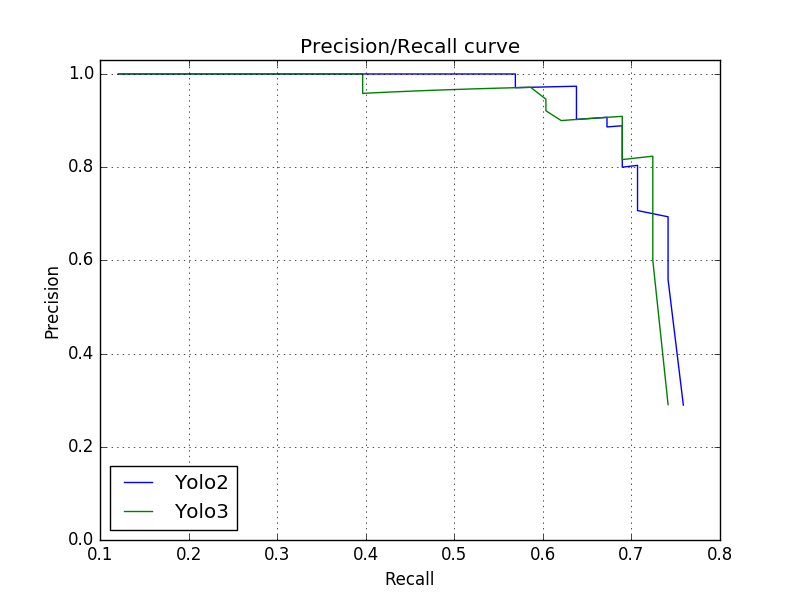
\includegraphics[width=0.8\linewidth]{results/case_buildings/prec_recall/yolo/bb.png}
  \caption{Yolo tested on bbnb}
  \label{fig:sfig1}
\end{subfigure}%
\begin{subfigure}{.5\textwidth}
  \centering
  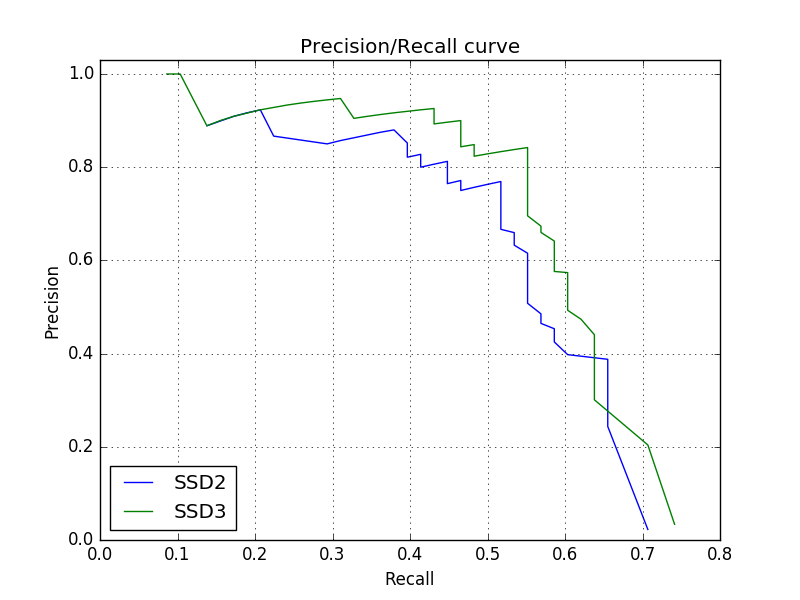
\includegraphics[width=.8\linewidth]{results/case_buildings/prec_recall/ssd/bb.png}
  \caption{SSD tested on bbnb}
  \label{fig:sfig2}
\end{subfigure}

\begin{subfigure}{.5\textwidth}
  \centering
  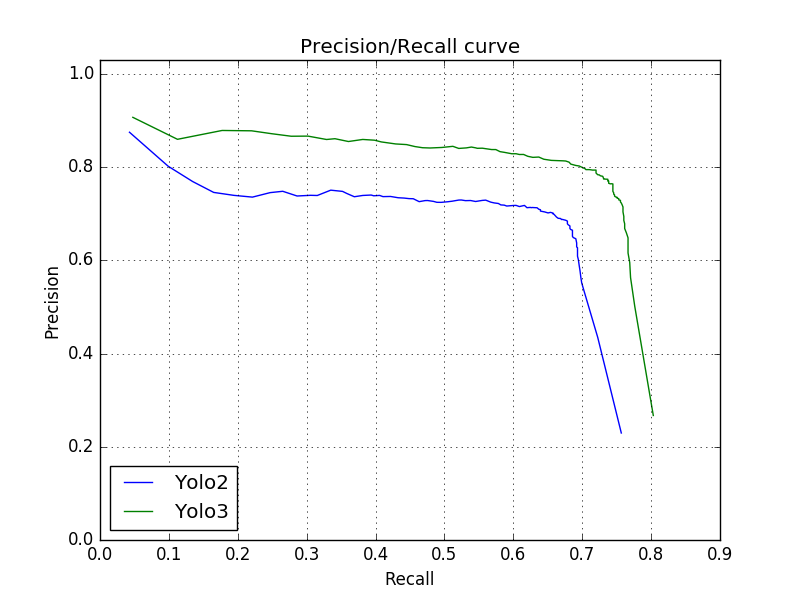
\includegraphics[width=0.8\linewidth]{results/case_buildings/prec_recall/yolo/bcbf.png}
  \caption{Yolo tested on bc, bf}
  \label{fig:sfig1}
\end{subfigure}%
\begin{subfigure}{.5\textwidth}
  \centering
  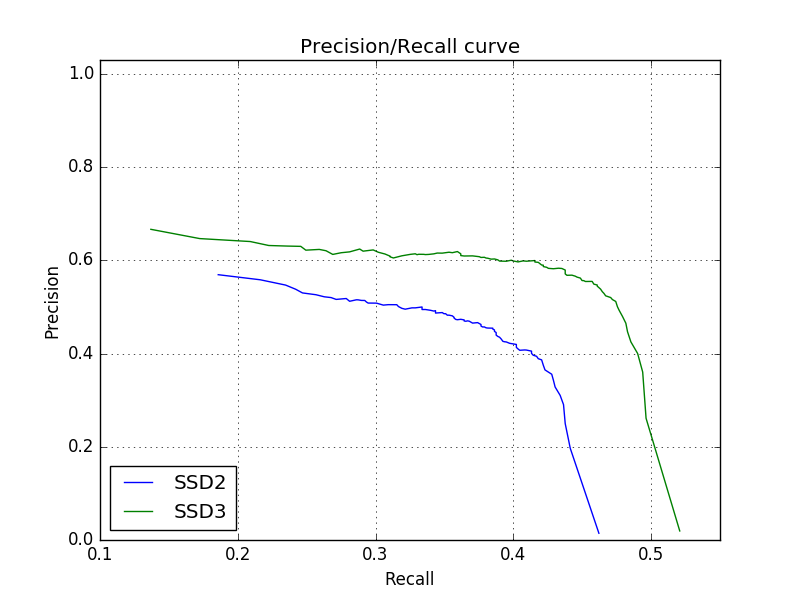
\includegraphics[width=.8\linewidth]{results/case_buildings/prec_recall/ssd/bcbf.png}
  \caption{SSD tested on bc, bf}
  \label{fig:sfig2}
\end{subfigure}

\begin{subfigure}{.5\textwidth}
  \centering
  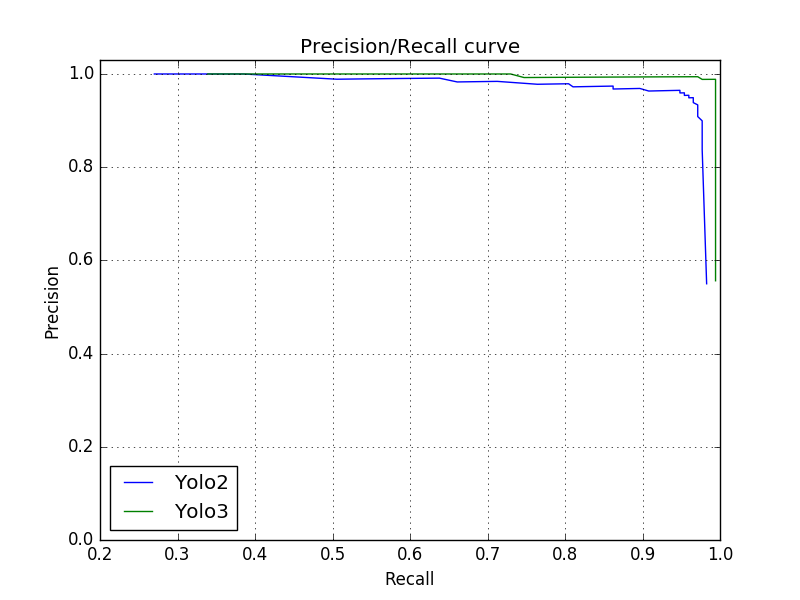
\includegraphics[width=0.8\linewidth]{results/case_buildings/prec_recall/yolo/trf.png}
  \caption{Yolo tested on trf}
  \label{fig:sfig1}
\end{subfigure}%
\begin{subfigure}{.5\textwidth}
  \centering
  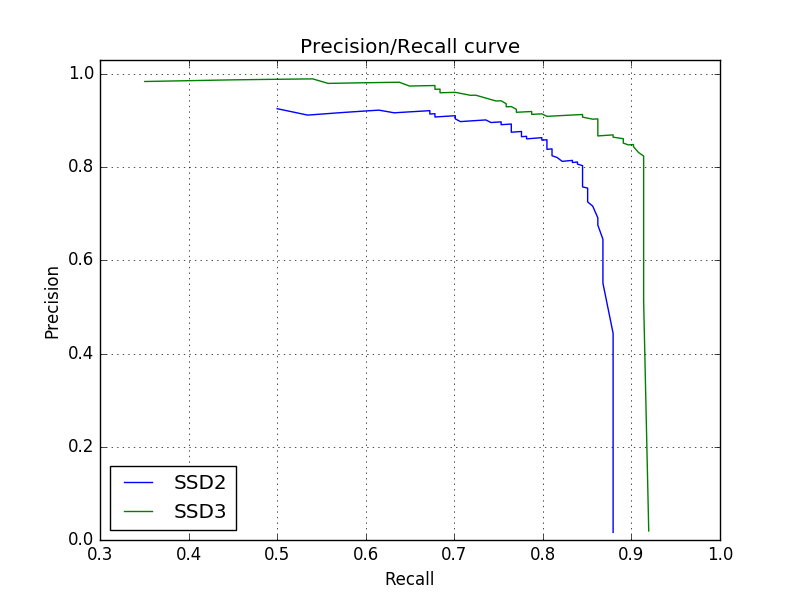
\includegraphics[width=.8\linewidth]{results/case_buildings/prec_recall/ssd/trf.png}
  \caption{SSD tested on trf}
  \label{fig:sfig2}
\end{subfigure}

\begin{subfigure}{.5\textwidth}
  \centering
  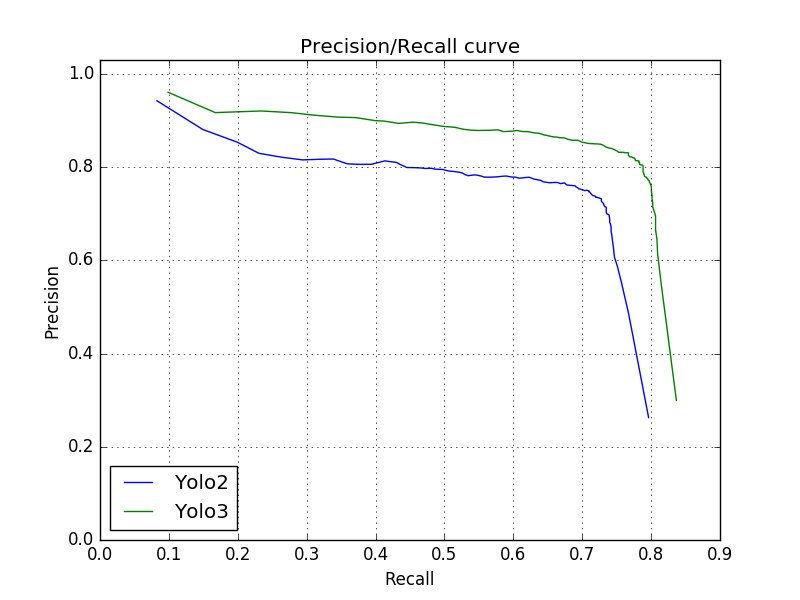
\includegraphics[width=0.8\linewidth]{results/case_buildings/prec_recall/yolo/bcbftrf.png}
  \caption{Yolo tested on bd, bf, trf}
  \label{fig:sfig1}
\end{subfigure}%
\begin{subfigure}{.5\textwidth}
  \centering
  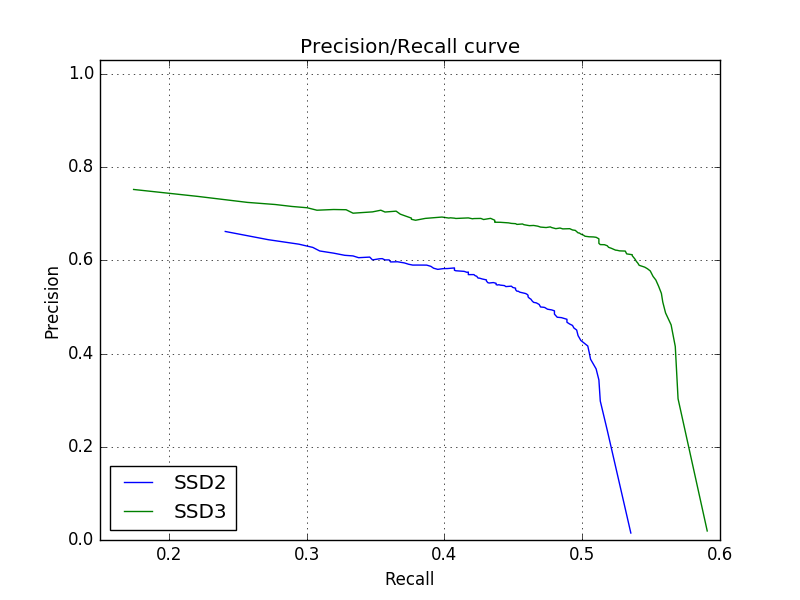
\includegraphics[width=.8\linewidth]{results/case_buildings/prec_recall/ssd/bcbftrf.png}
  \caption{SSD tested on bc, bf, trf}
  \label{fig:sfig2}
\end{subfigure}
\caption{Precision/recall curves of Yolo2, Yolo3, SSD2 and SSD3}
\label{fig:case_build}
\end{figure}

\newpage

\subsection{Tested on bbnb}

The hypothesis before running the experiment was that the bbnb dataset would be the most postively affected by training on a building class. Since \textit{bbnb} consists of mostly moored boats, where there are images that contain buildings close to sea level one could suspect could be mistaken as boats, as shown in \ref{img:bbnb_ex}. The building in the bottom left corner is close to sea level, while also being relatively close in size to the boats compared to the other buildings in the image, which makes it a good candidate for a misclassification. However, neither Yolo2 nor SSD2 classifies this building as a boat. All the detectors, Yolo2, Yolo3, SSD2 and SSD3 detects all the boats in the image. Both SSD2 and SSD3 detects the rightmost boat two times, and the bounding box differences between Yolo2 and Yolo3 and between SSD2 and SSD3 are so insignificant that training on the building class does not seem to help improve performance on this particular image. Both Yolo3 and ssd3 detects the buildings in the image well, as can be seen in figure \ref{fig:ex_bbnb_yolo3} and \ref{fig:ex_bbnb_ssd3}.


\begin{figure}[h!]
\begin{subfigure}{.5\textwidth}
  \centering
  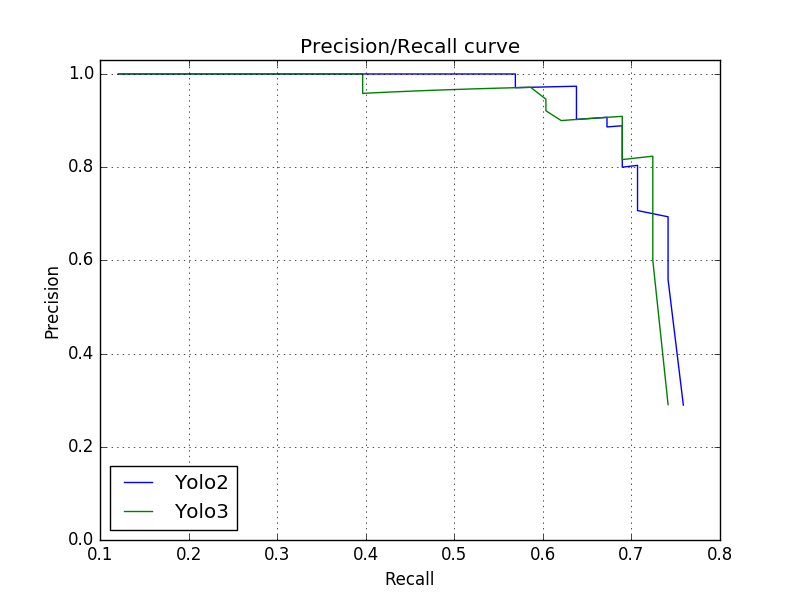
\includegraphics[width=0.8\linewidth]{results/case_buildings/prec_recall/yolo/bb.png}
  \caption{Yolo tested on bbnb}
  \label{fig:ex_bnbb_prec_rec_yolo}
\end{subfigure}%
\begin{subfigure}{.5\textwidth}
  \centering
  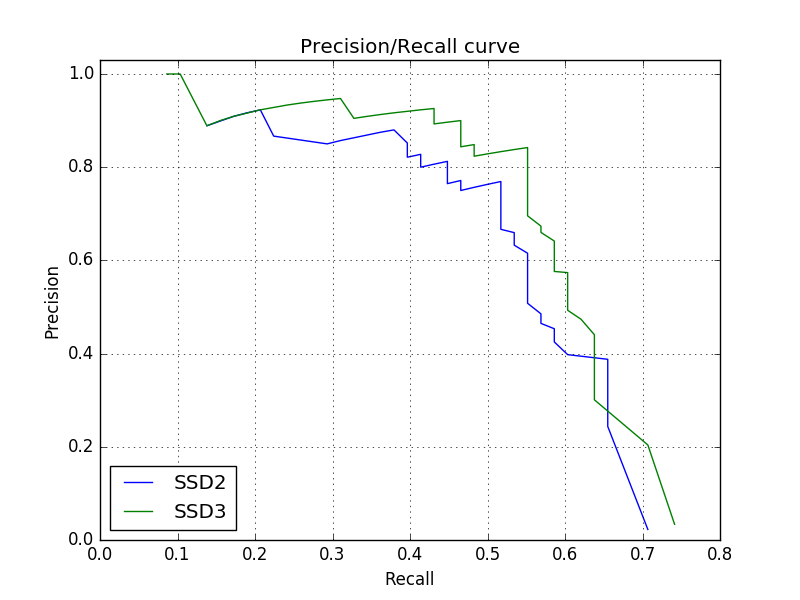
\includegraphics[width=.8\linewidth]{results/case_buildings/prec_recall/ssd/bb.png}
  \caption{SSD tested on bbnb}
  \label{fig:ex_bnbb_prec_rec_ssd}
\end{subfigure}
\begin{subfigure}{.5\textwidth}
  \centering
  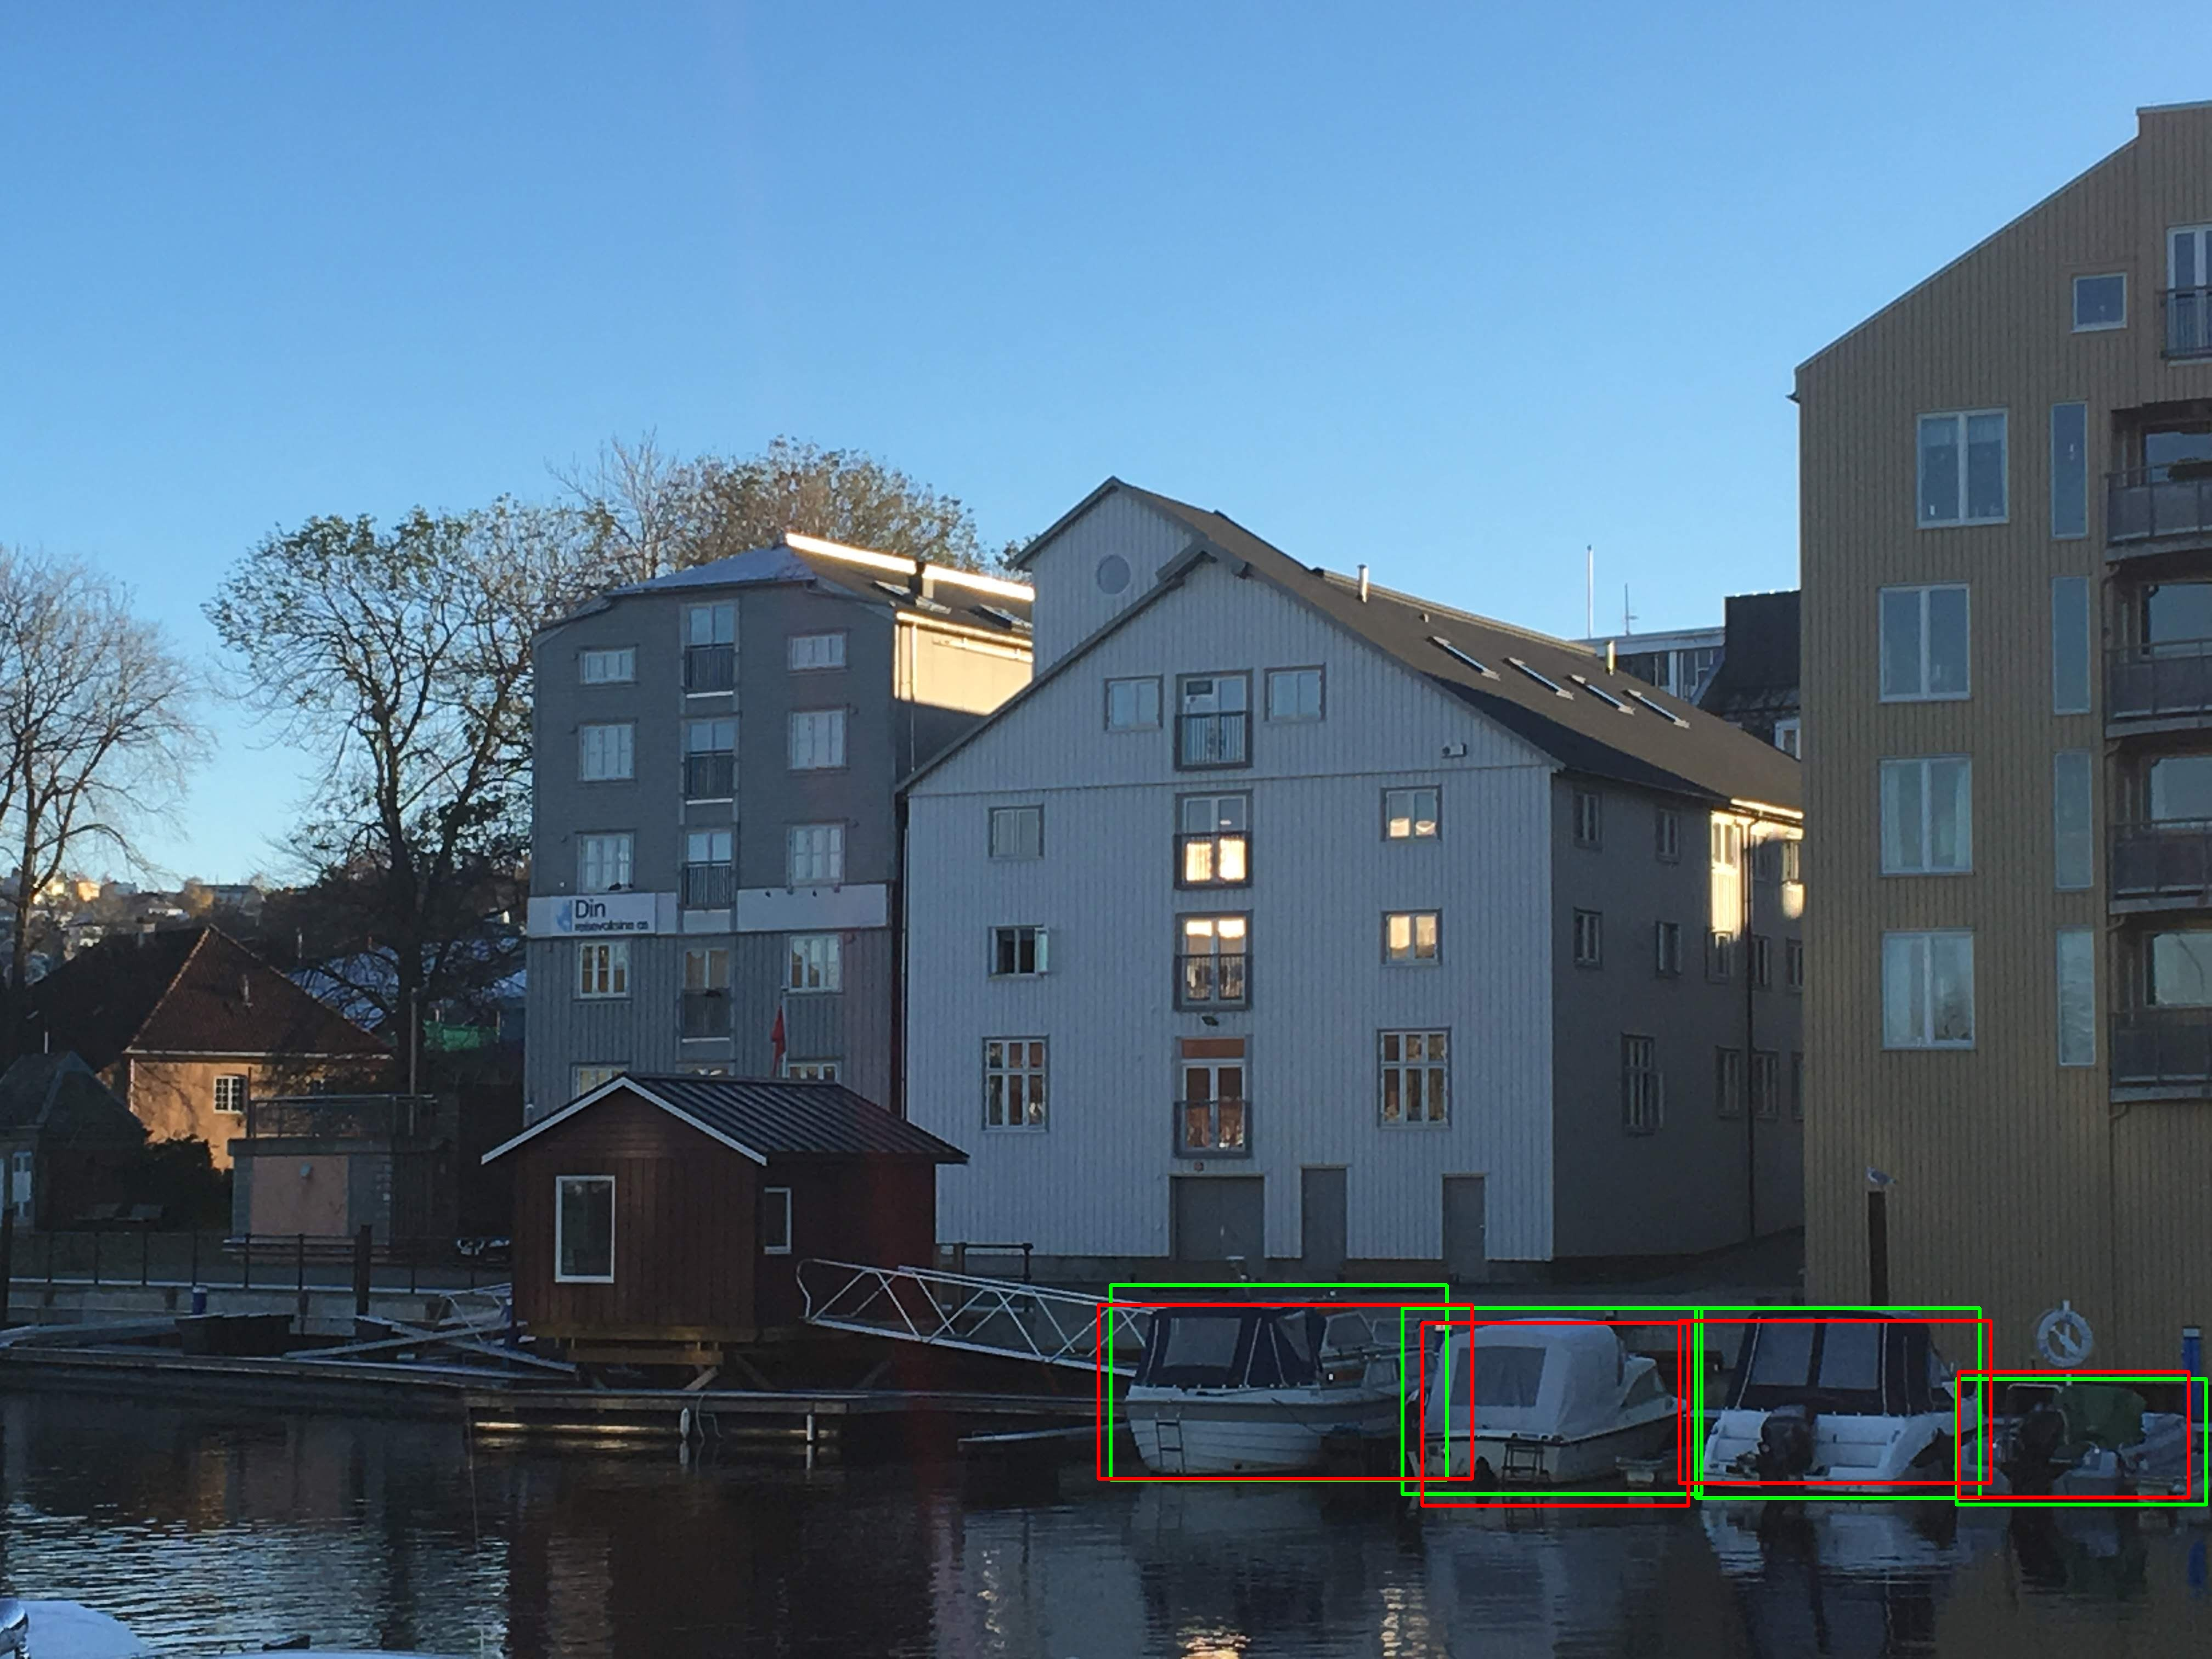
\includegraphics[width=0.8\linewidth]{results/case_buildings/prec_recall/yolo/IMG_2077_bbnb.jpg}
  \caption{Yolo2}
  \label{fig:ex_bbnb_yolo2}
\end{subfigure}%
\begin{subfigure}{.5\textwidth}
  \centering
  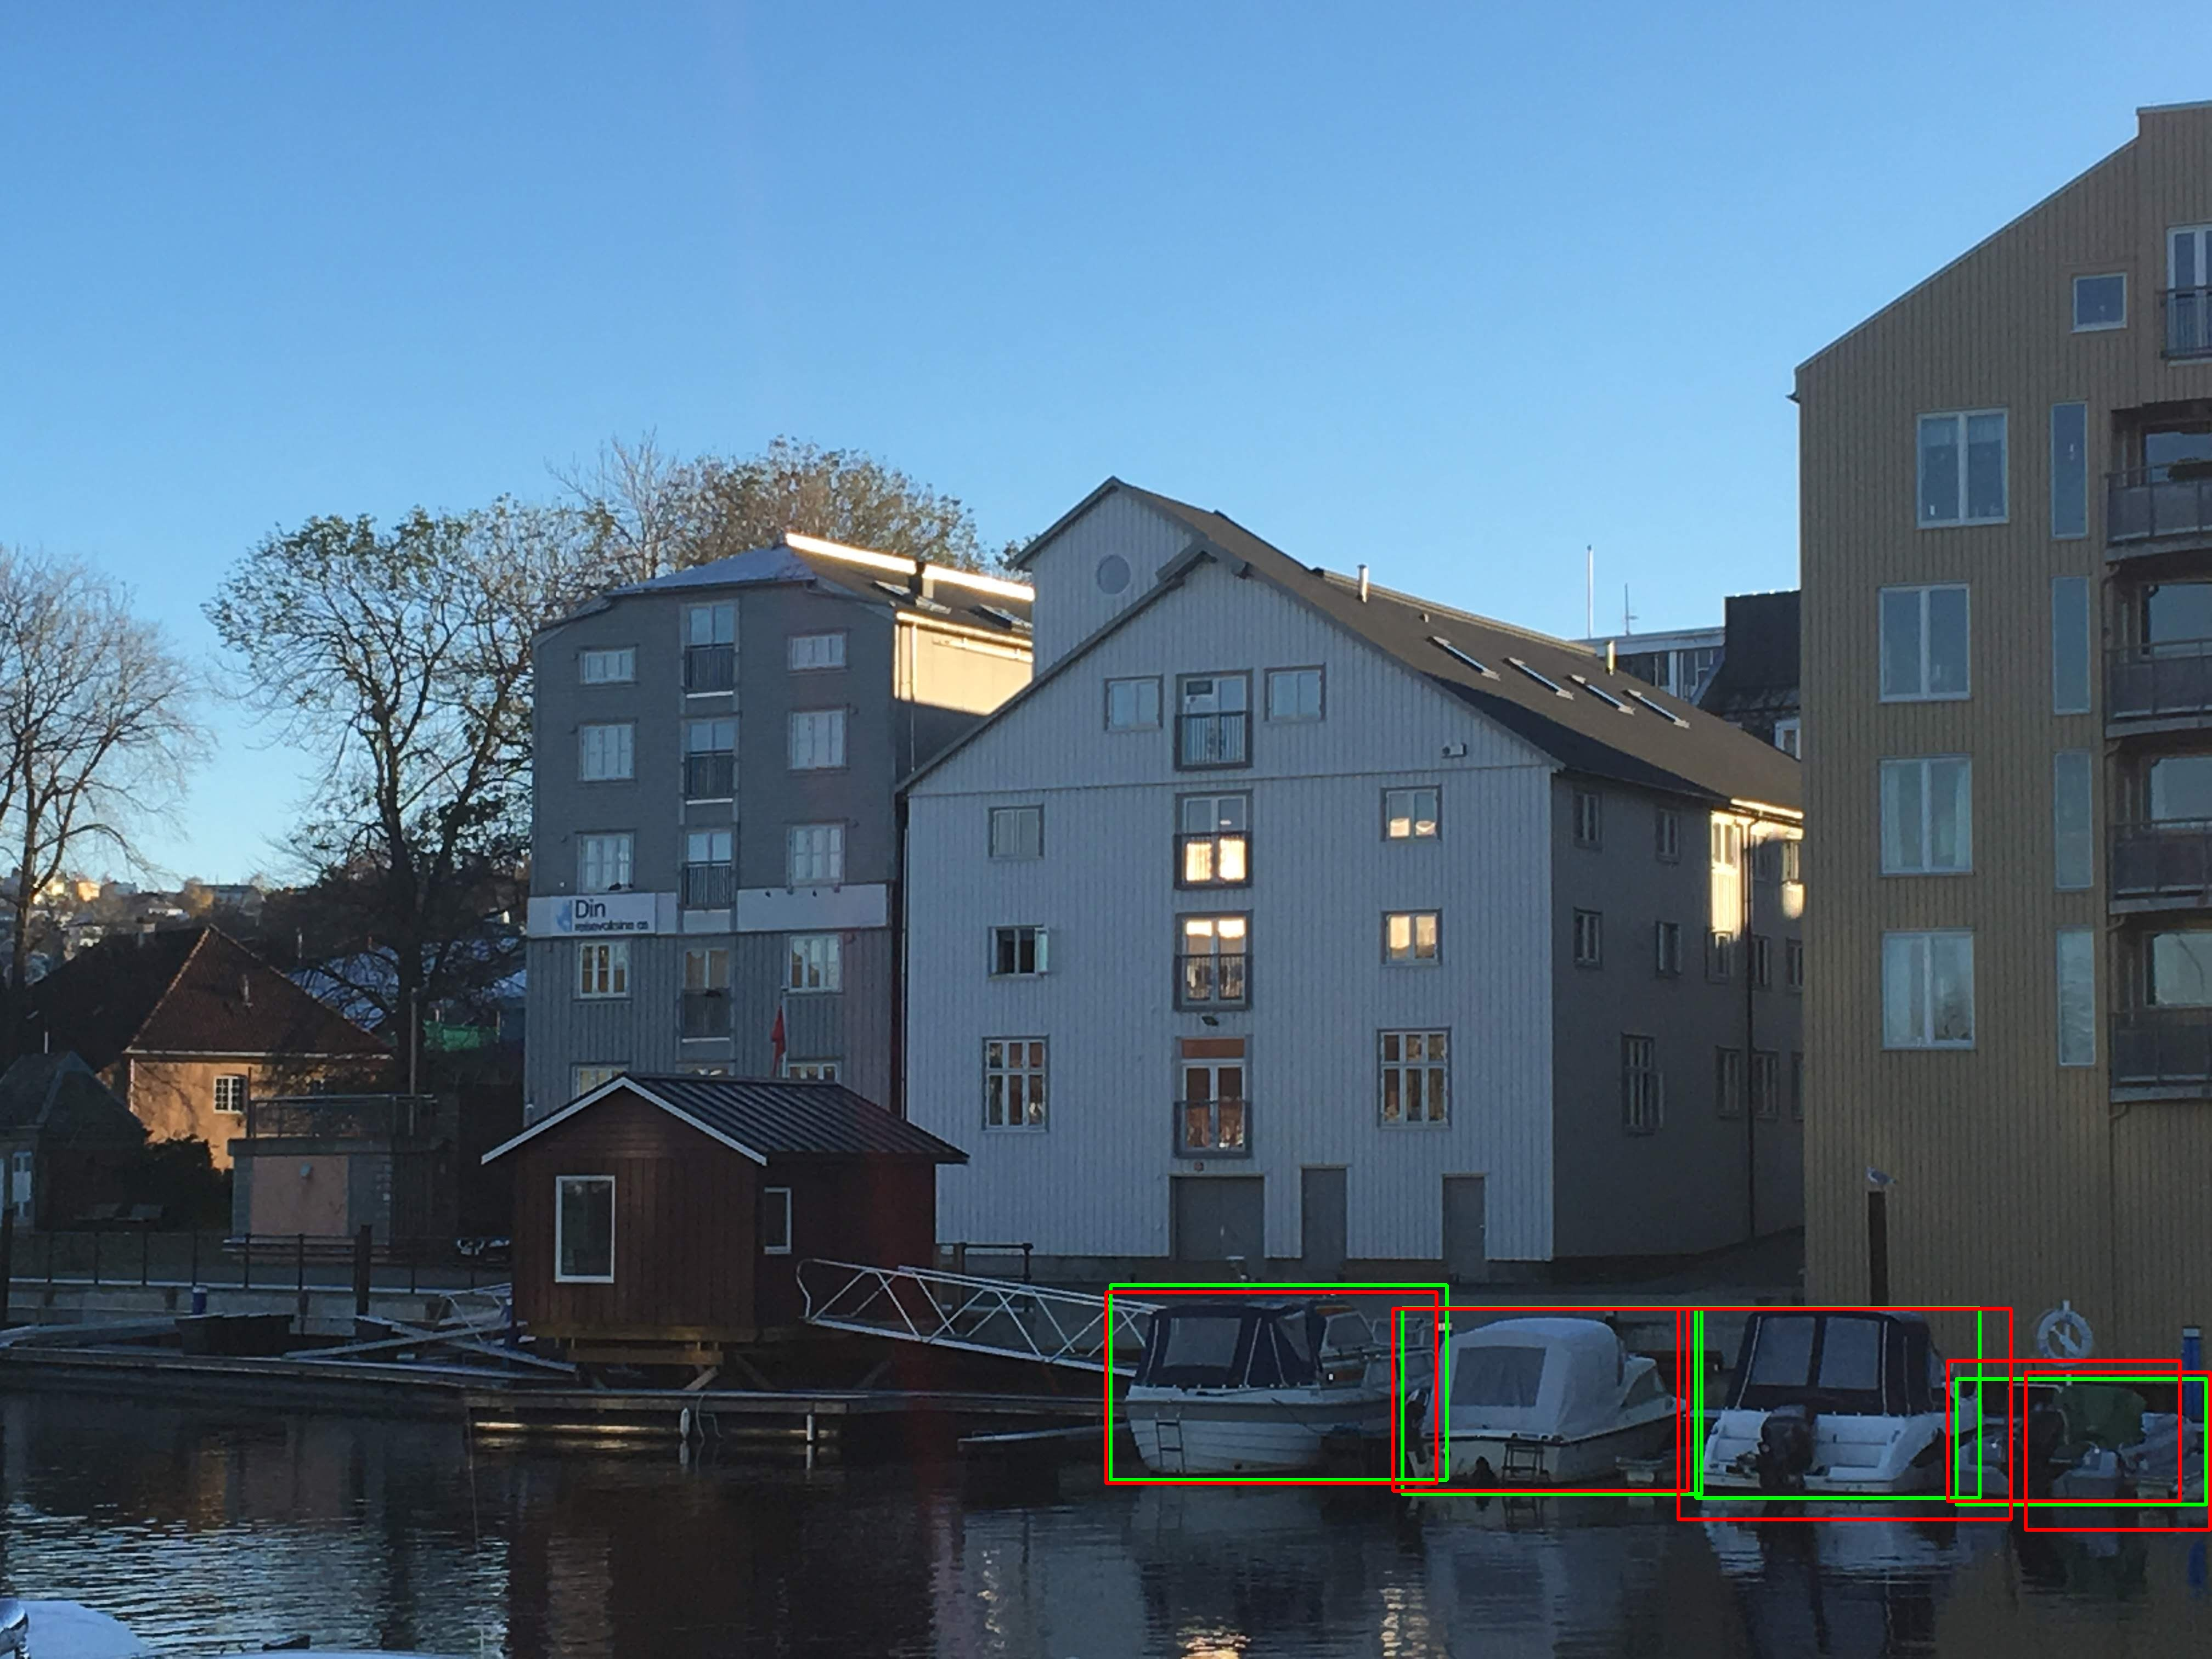
\includegraphics[width=.8\linewidth]{results/case_buildings/prec_recall/ssd/IMG_2077_bbnb.jpg}
  \caption{SSD2}
  \label{fig:ex_bbnb_ssd2}
\end{subfigure}

\begin{subfigure}{.5\textwidth}
  \centering
  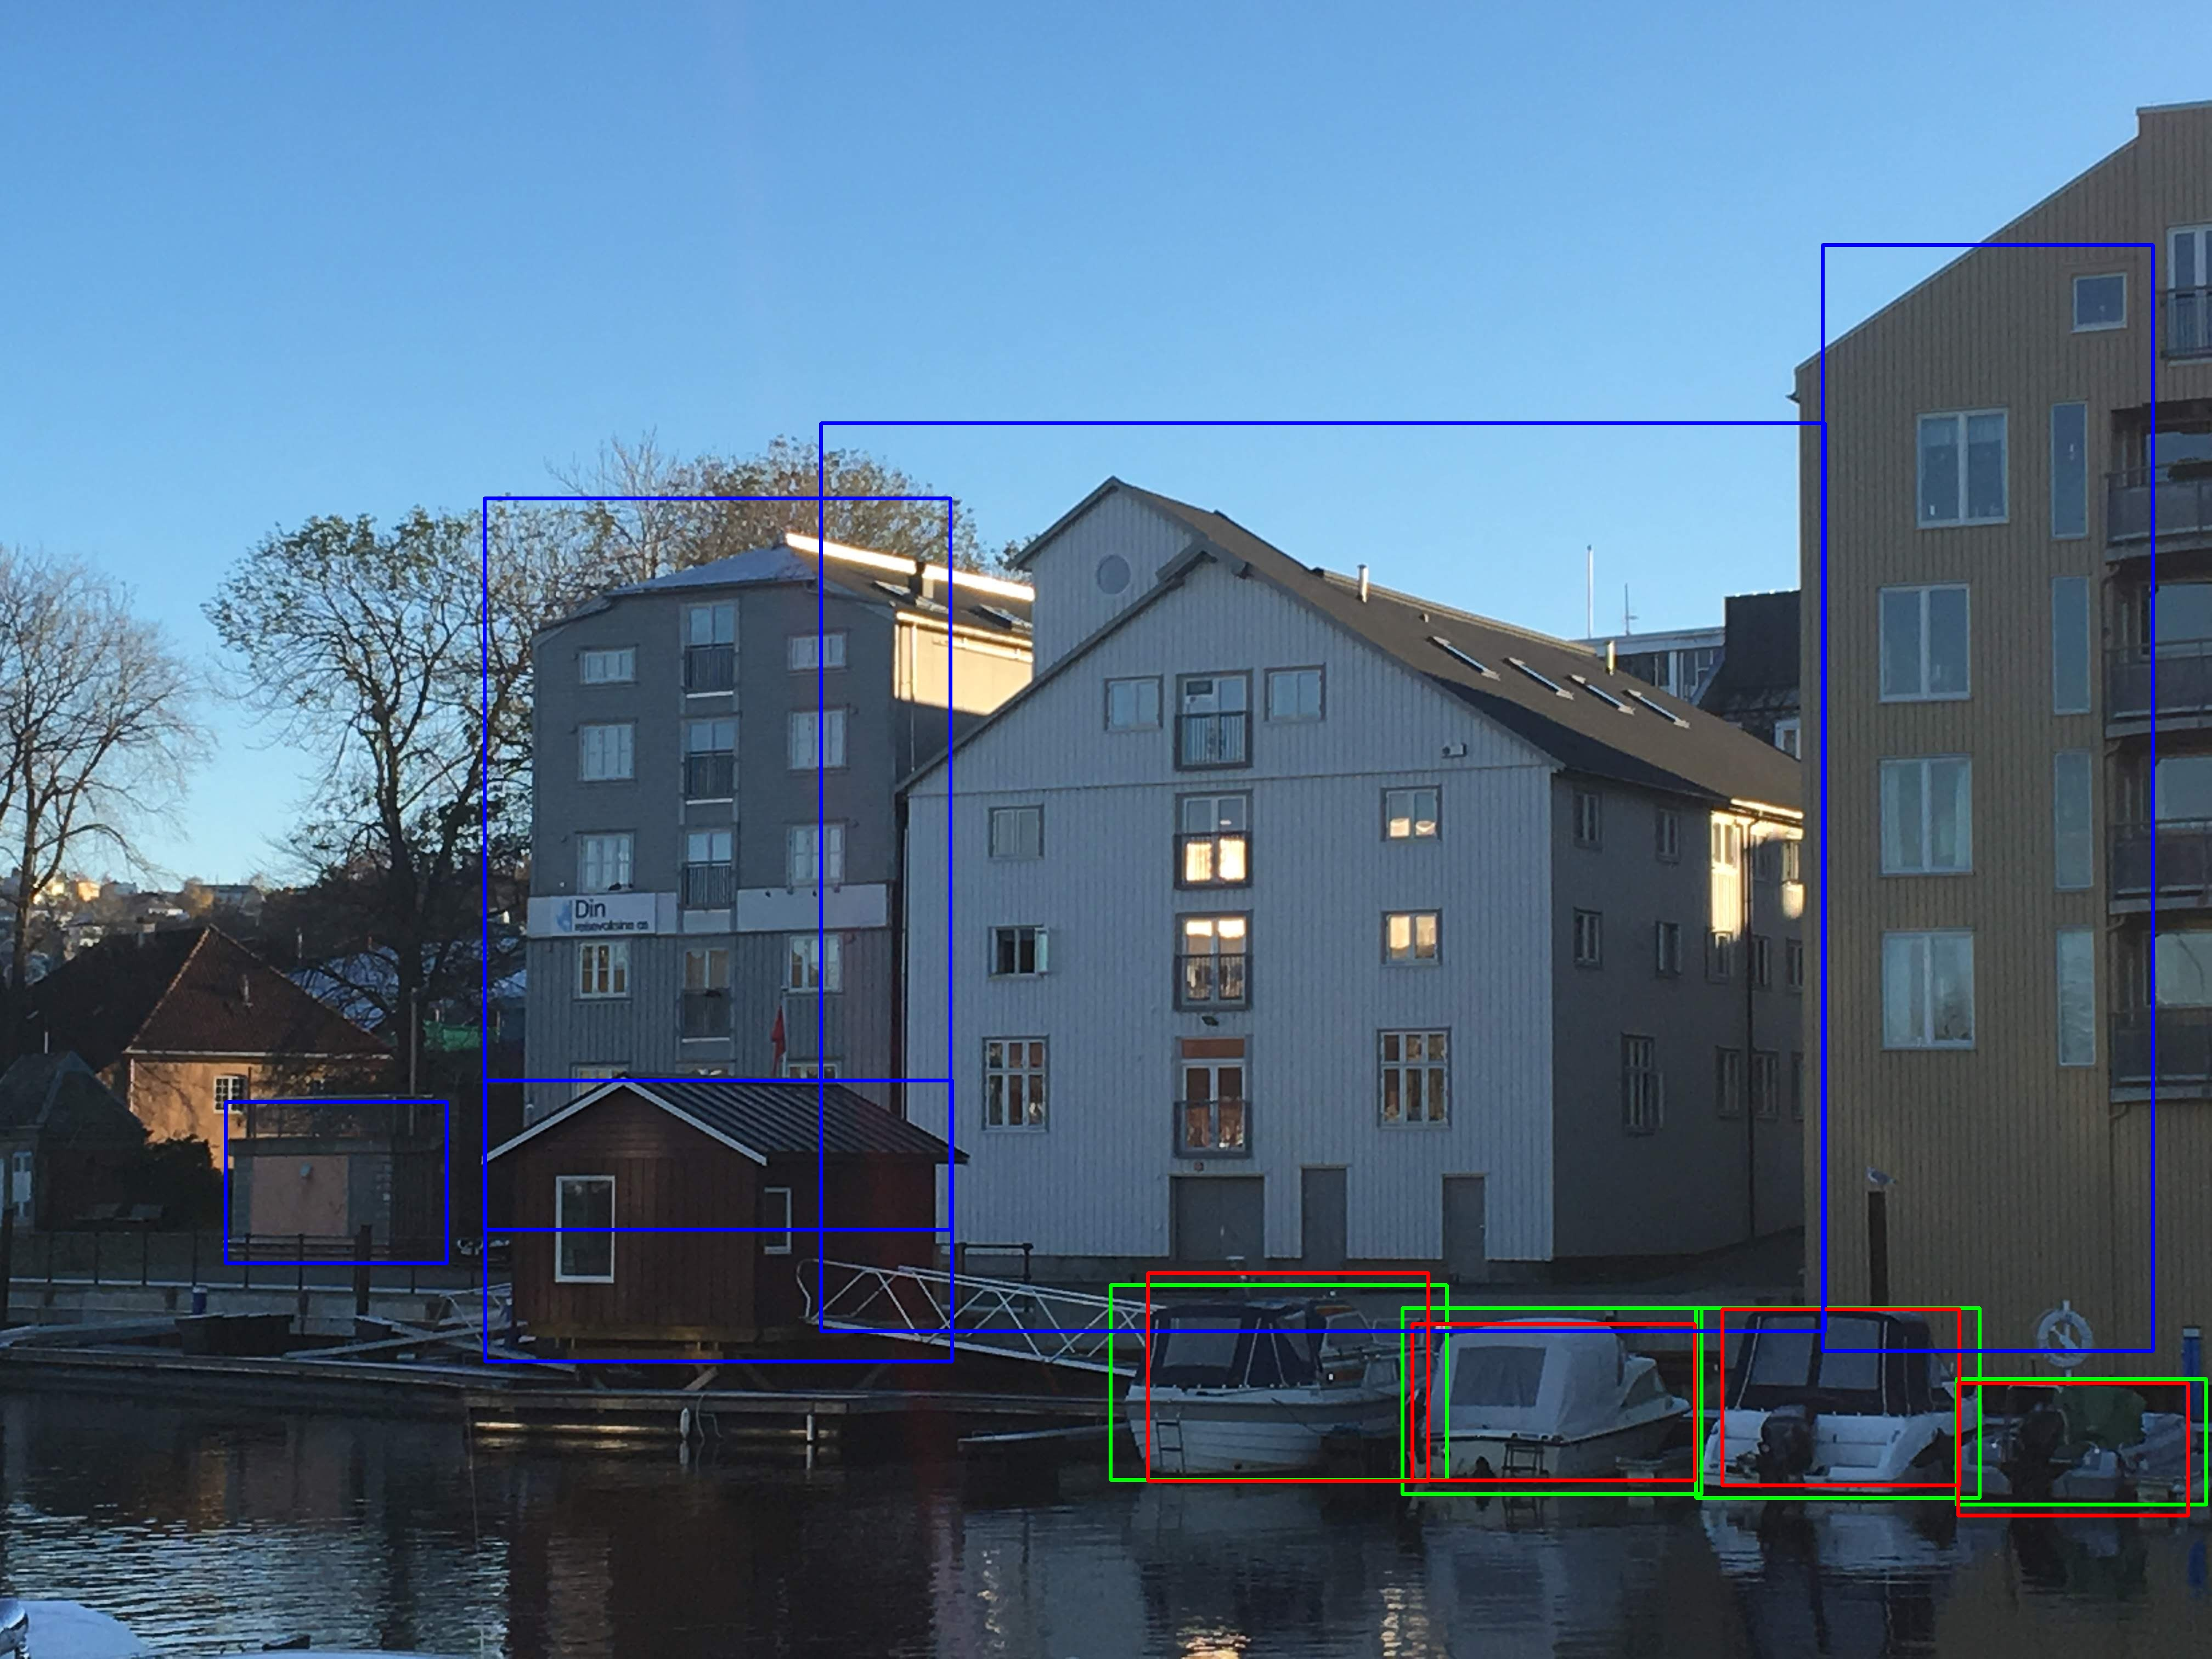
\includegraphics[width=0.8\linewidth]{results/case_buildings/prec_recall/yolo/IMG_2077_build.jpg}
  \caption{Yolo3}
  \label{fig:ex_bbnb_yolo3}
\end{subfigure}%
\begin{subfigure}{.5\textwidth}
  \centering
  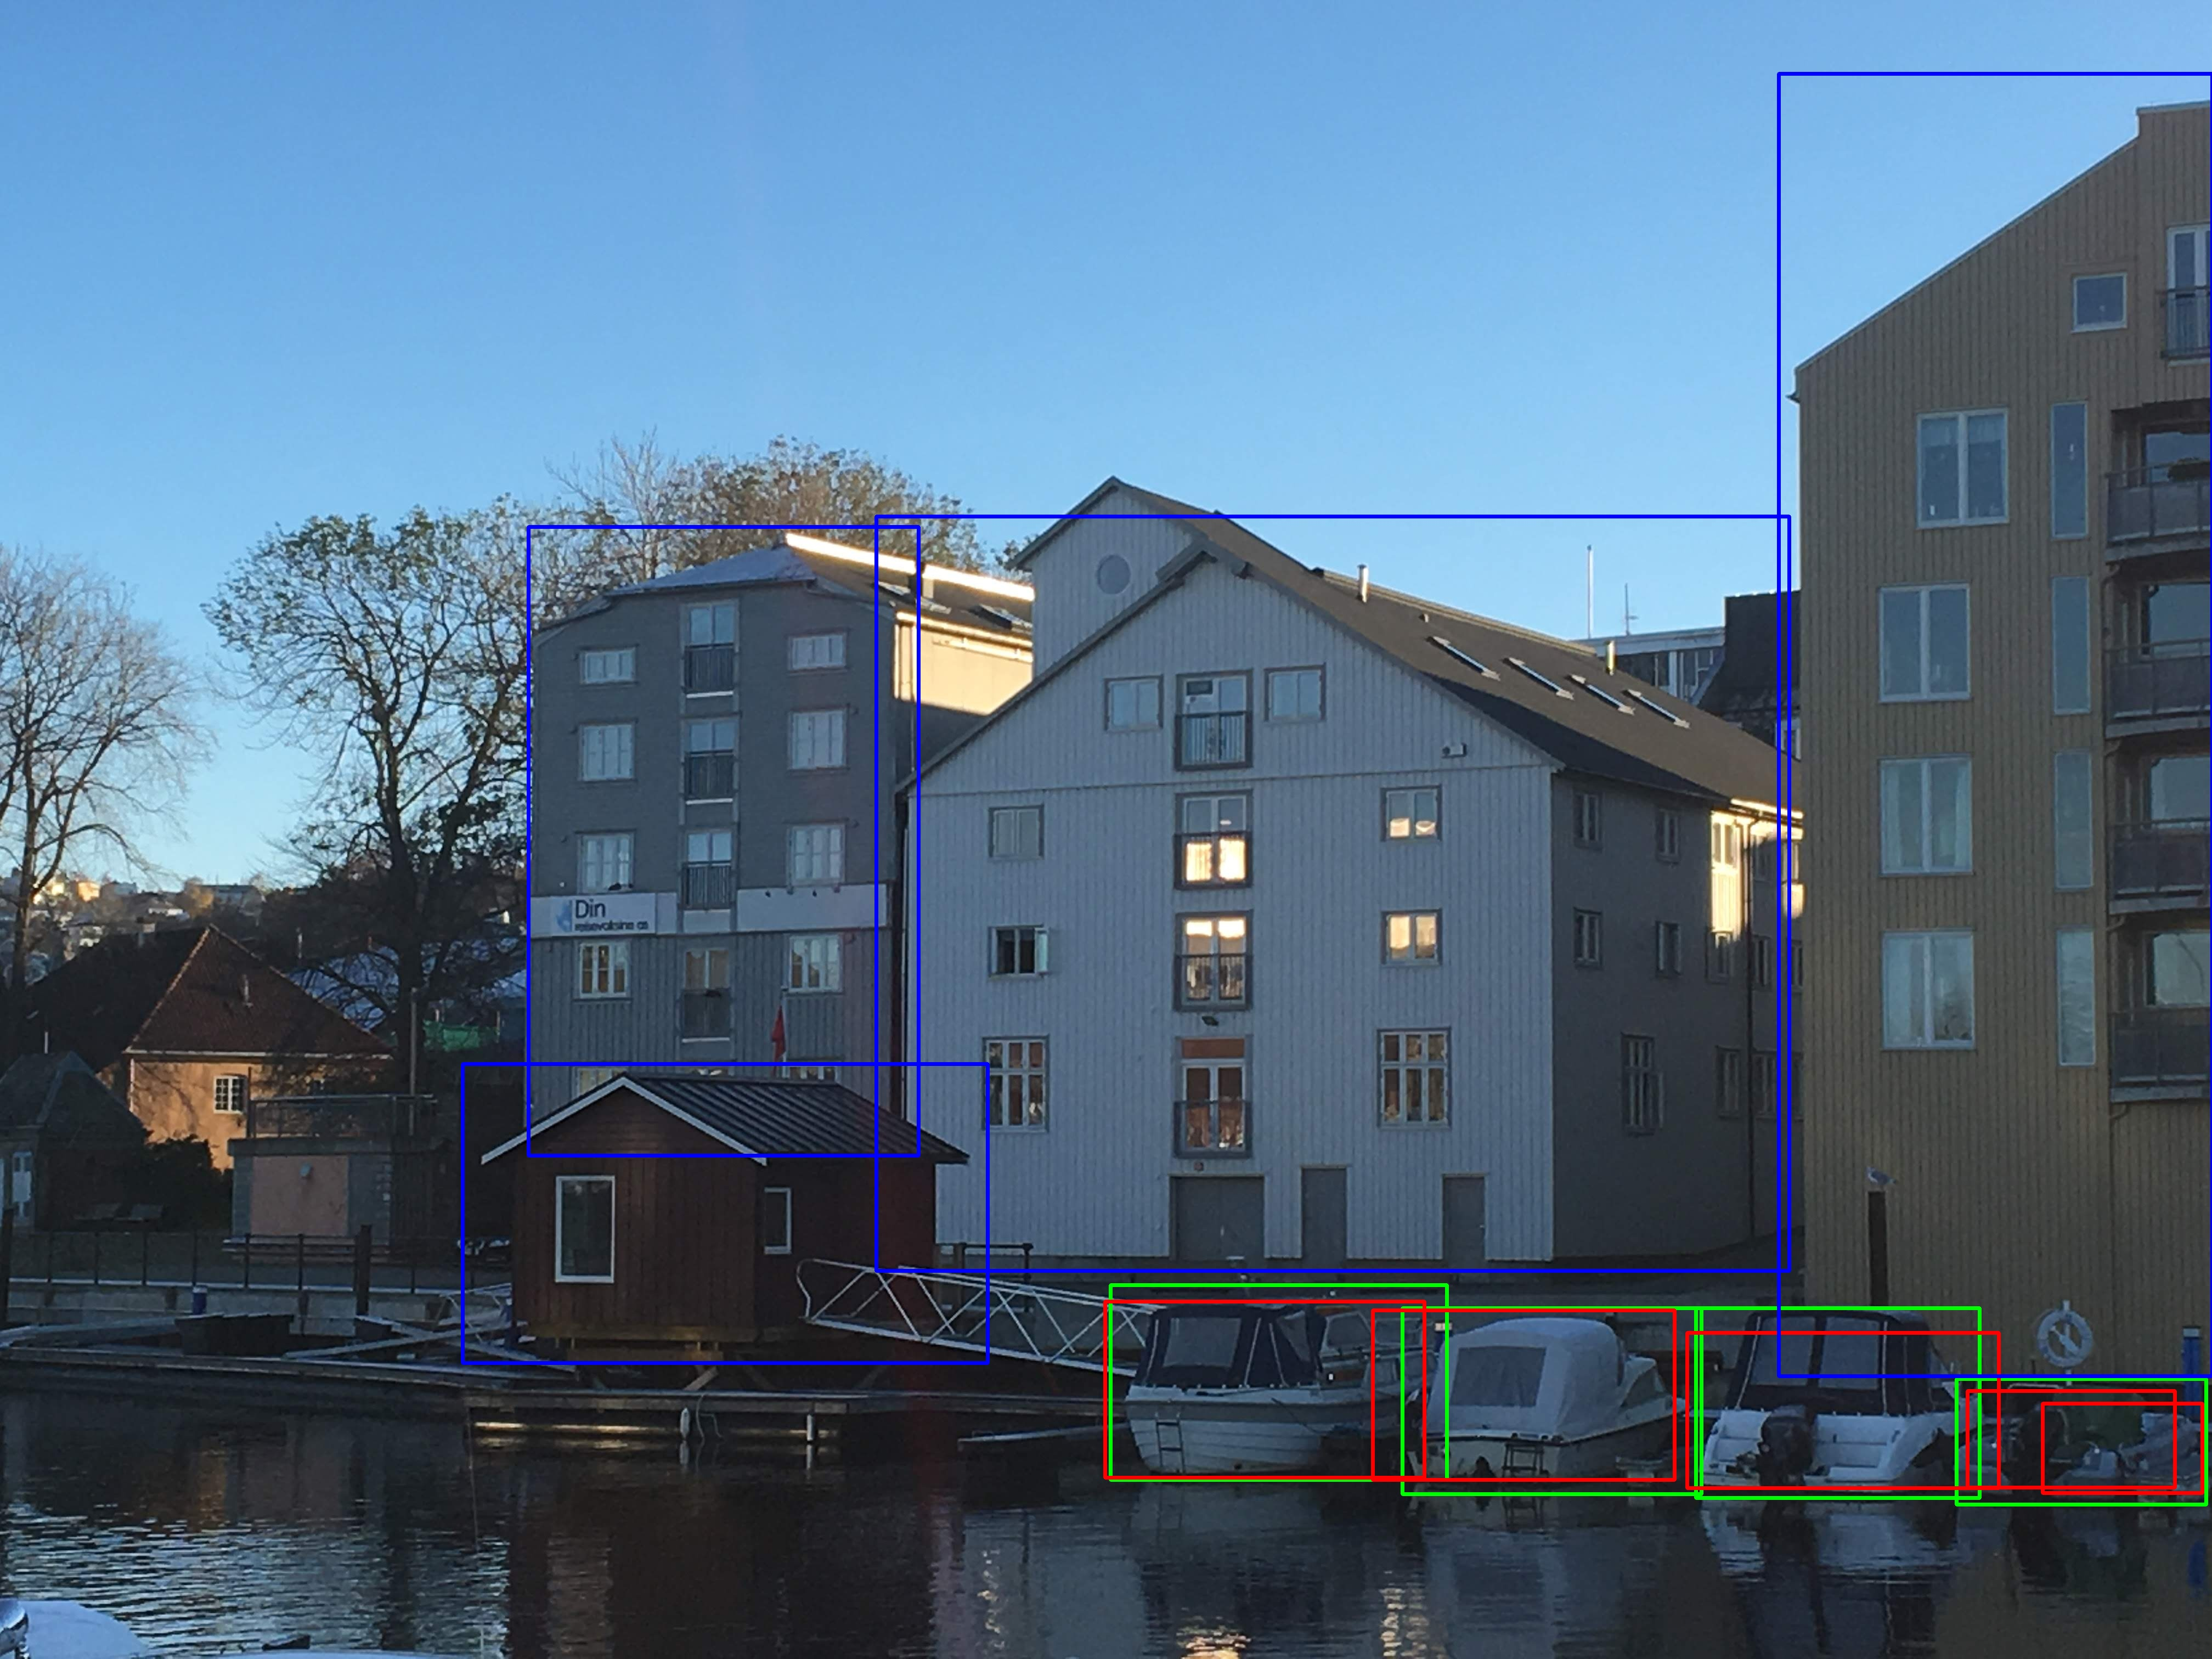
\includegraphics[width=.8\linewidth]{results/case_buildings/prec_recall/ssd/IMG_2077_build.jpg}
  \caption{SSD3}
  \label{fig:ex_bbnb_ssd3}
\end{subfigure}
\caption{Yolo2, Yolo3, SSD2, SSD3 example image from \textit{bbnb} test set. Green bounding boxes are ground truth, red bounding boxes are detected boats, blue bounding boxes are detected buildings}
\label{img:bbnb_ex}
\end{figure}

\newpage

\subsection{Tested on bc, bf}

The datasets \textit{bc} and \textit{bf} consists mostly of images taken towards open sea, of boats that are sailing, i.e. the boats are not moored. It is on this dataset the performance differences between Yolo2 and Yolo3 and between SSD2 and SSD3 differ the most, as can be seen in figure \ref{fig:case_build}.

\vspace{3mm}

By going through the 300 test images some differences between the models become apparent. While the differences between SSD2 and SSD3 are somewhat obvious, the difference between Yolo2 and Yolo3 are more nuanced. Around 10 percent of the test images SSD2 detects land as a boat, in none of these images does SSD3 perform the same way. An example of this is shown in figure \ref{img:bixbox_ssd}. More examples of this behaviour can be found in appendix C in chapter \ref{sec:bigbox}

\begin{figure}[h!]
\begin{subfigure}{.5\textwidth}
  \centering
  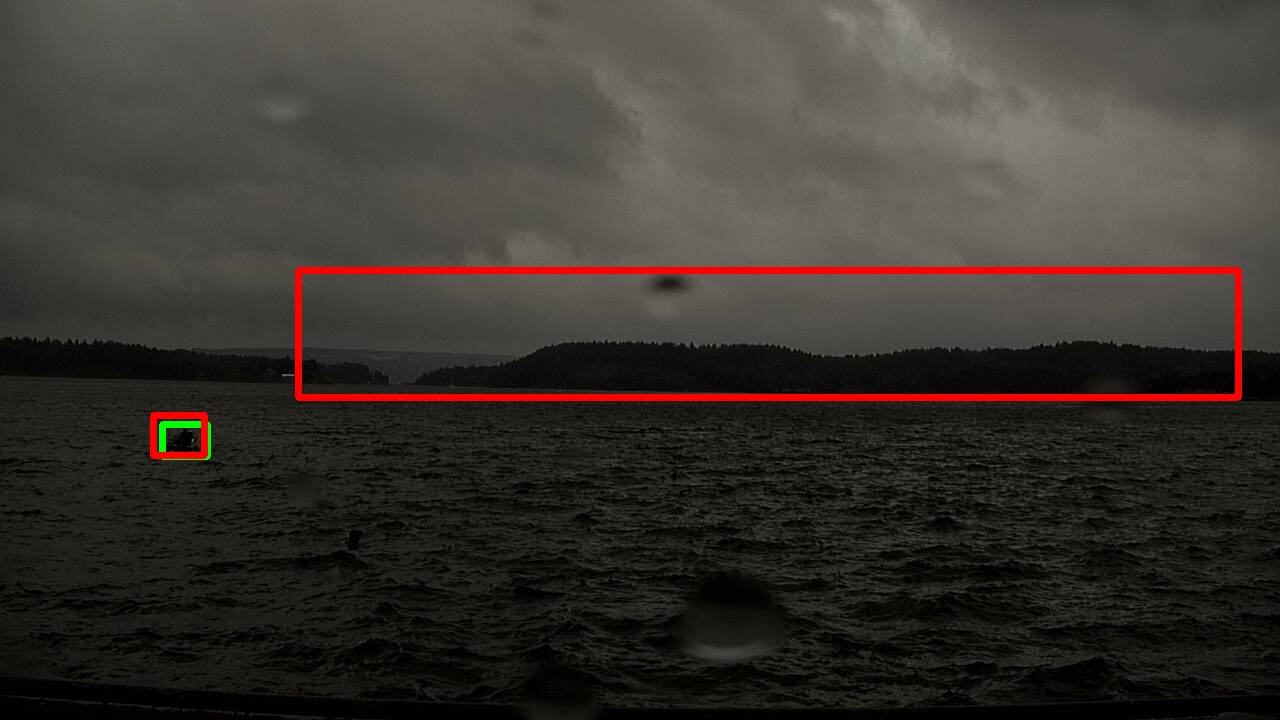
\includegraphics[width=0.9\linewidth]{results/case_buildings/bigbox_bcbf/SSD2/selected_06_14_axis0049.jpg}
  \caption{SSD2}
  \label{fig:big_box_ssd2}
\end{subfigure}%
\begin{subfigure}{.5\textwidth}
  \centering
  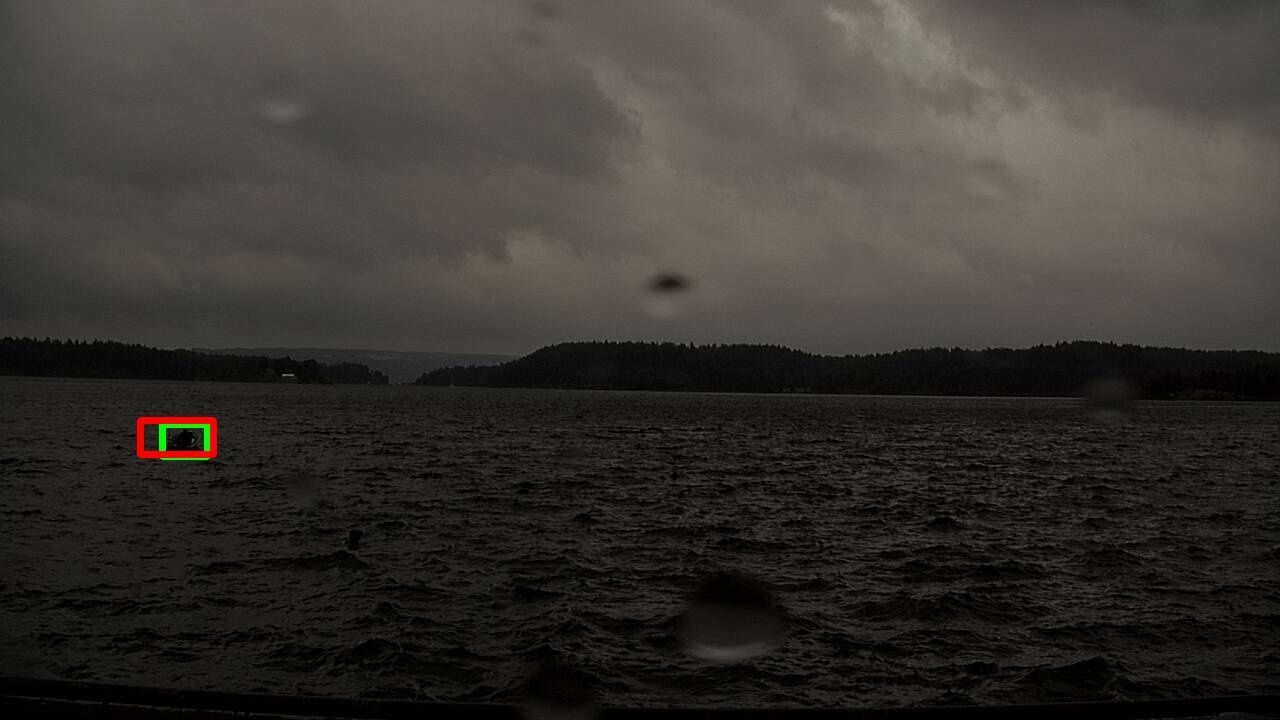
\includegraphics[width=.9\linewidth]{results/case_buildings/bigbox_bcbf/SSD3/selected_06_14_axis0049.jpg}
  \caption{SSD3}
  \label{fig:big_box_ssd3}
\end{subfigure}
\caption{SSD2 detects land as boat. Red bounding boxes are boat detections, green bounding boxes are ground truth.}
\label{img:bixbox_ssd}
\end{figure}

There are also some examples where SSD2 misclassifies buildings as boats, while SSD3 does not. One example is shown in 

\begin{figure}[h!]
\begin{subfigure}{.5\textwidth}
  \centering
  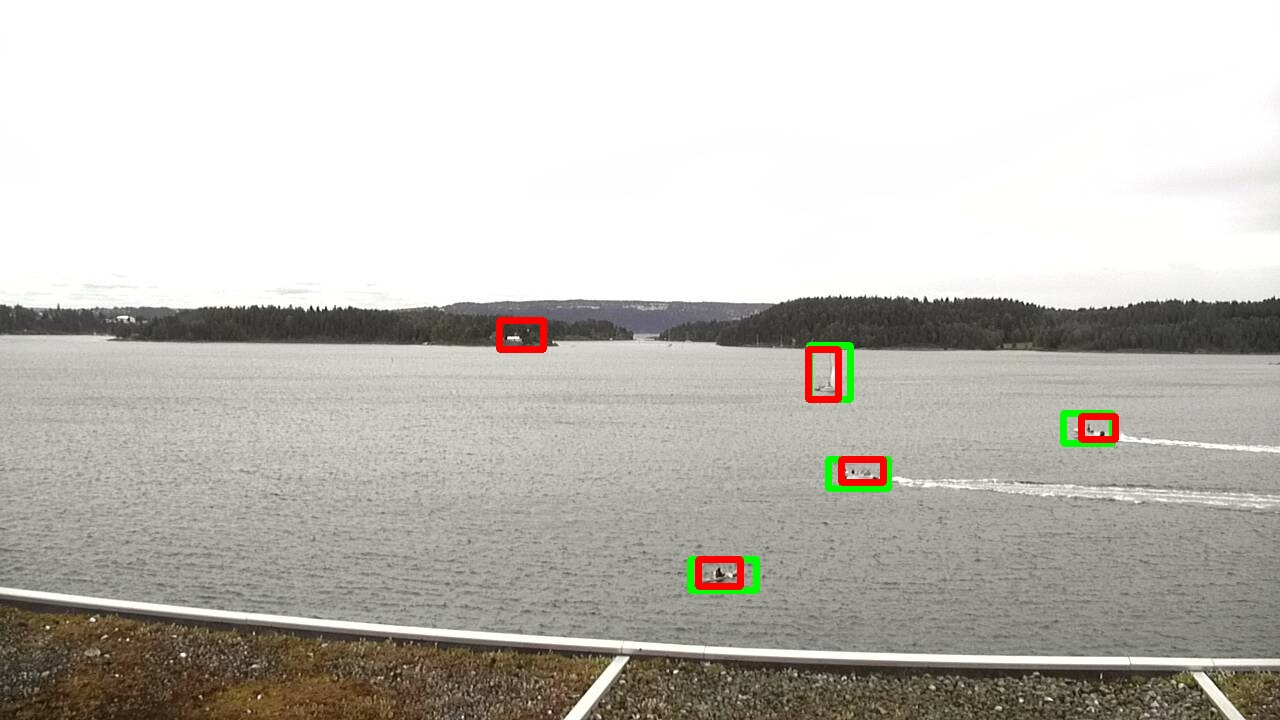
\includegraphics[width=0.9\linewidth]{results/case_buildings/misclass/selected_08_07_frame11982_bbnb.jpg}
  \caption{SSD2}
  \label{fig:misclass_ssd2}
\end{subfigure}%
\begin{subfigure}{.5\textwidth}
  \centering
  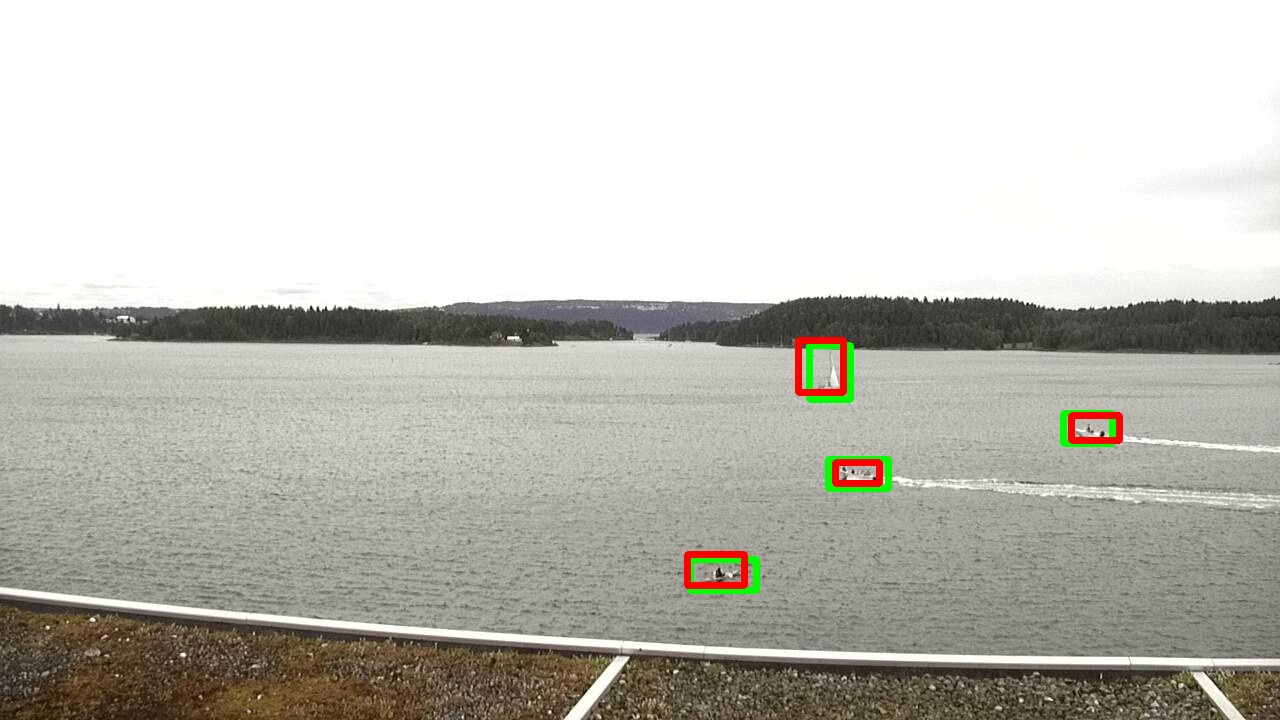
\includegraphics[width=.9\linewidth]{results/case_buildings/misclass/selected_08_07_frame11982_build.jpg}
  \caption{SSD3}
  \label{fig:misclass_ssd3}
\end{subfigure}
\caption{Leftmost red bounding box in SSD2 is a detection of a building as a boat, this is not detected as a boat in SSD3. Red bounding boxes are boat detections, green bounding boxes are ground truth.}
\label{img:misclass_ssd}
\end{figure}

\vspace{3mm}

As mentioned Yolo2 and Yolo3 does not differ as clearly as SSD2 and SSD3. There are examples of Yolo2 performing better than Yolo3 and vice versa. In many of the misclassifications in the test data both Yolo2 and Yolo3 mistakes the same object as a boat. By analysing the results from both Yolo2 and Yolo3 the following conclusions can be drawn:

\begin{itemize}
    \item Yolo2 and Yolo3 has a tendency to mistake the same objects as boats. See Appendix C chapter \ref{sec:same_mistake} for example images.
    \item Yolo2 performs better in some cases, while Yolo3 performs better in other. It is not clear what makes one better than the other in each specific case. See Appendix C chapter \ref{sec:3better} and \ref{sec:2better} for example images
    \item Yolo2 makes some misclassifications that could imply that training on a building class makes Yolo3 more robust to the more incomrehensible misclassifications. See appendix C chapter \ref{sec:yolo2_spec_misc} for example images.
\end{itemize}






\begin{figure}[h!]
\begin{subfigure}{.5\textwidth}
  \centering
  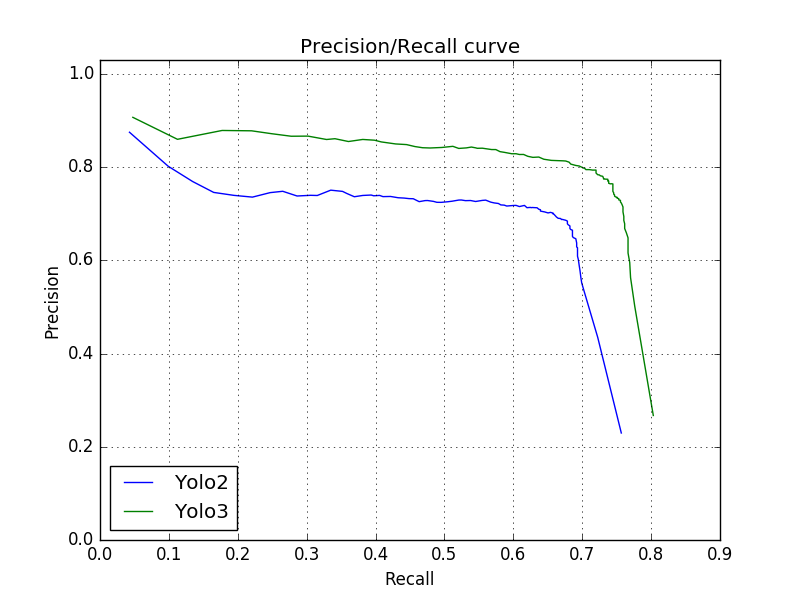
\includegraphics[width=0.8\linewidth]{results/case_buildings/prec_recall/yolo/bcbf.png}
  \caption{Yolo tested on bc, bf}
  \label{fig:ex_bcbf_prec_rec_yolo}
\end{subfigure}%
\begin{subfigure}{.5\textwidth}
  \centering
  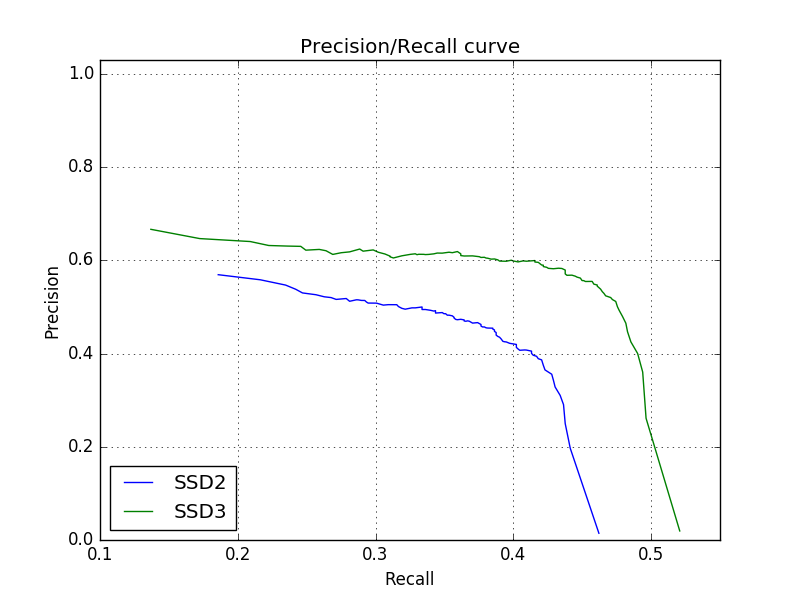
\includegraphics[width=.8\linewidth]{results/case_buildings/prec_recall/ssd/bcbf.png}
  \caption{SSD tested on bc, bf}
  \label{fig:ex_bcbf_prec_rec_ssd}
\end{subfigure}
\begin{subfigure}{.5\textwidth}
  \centering
  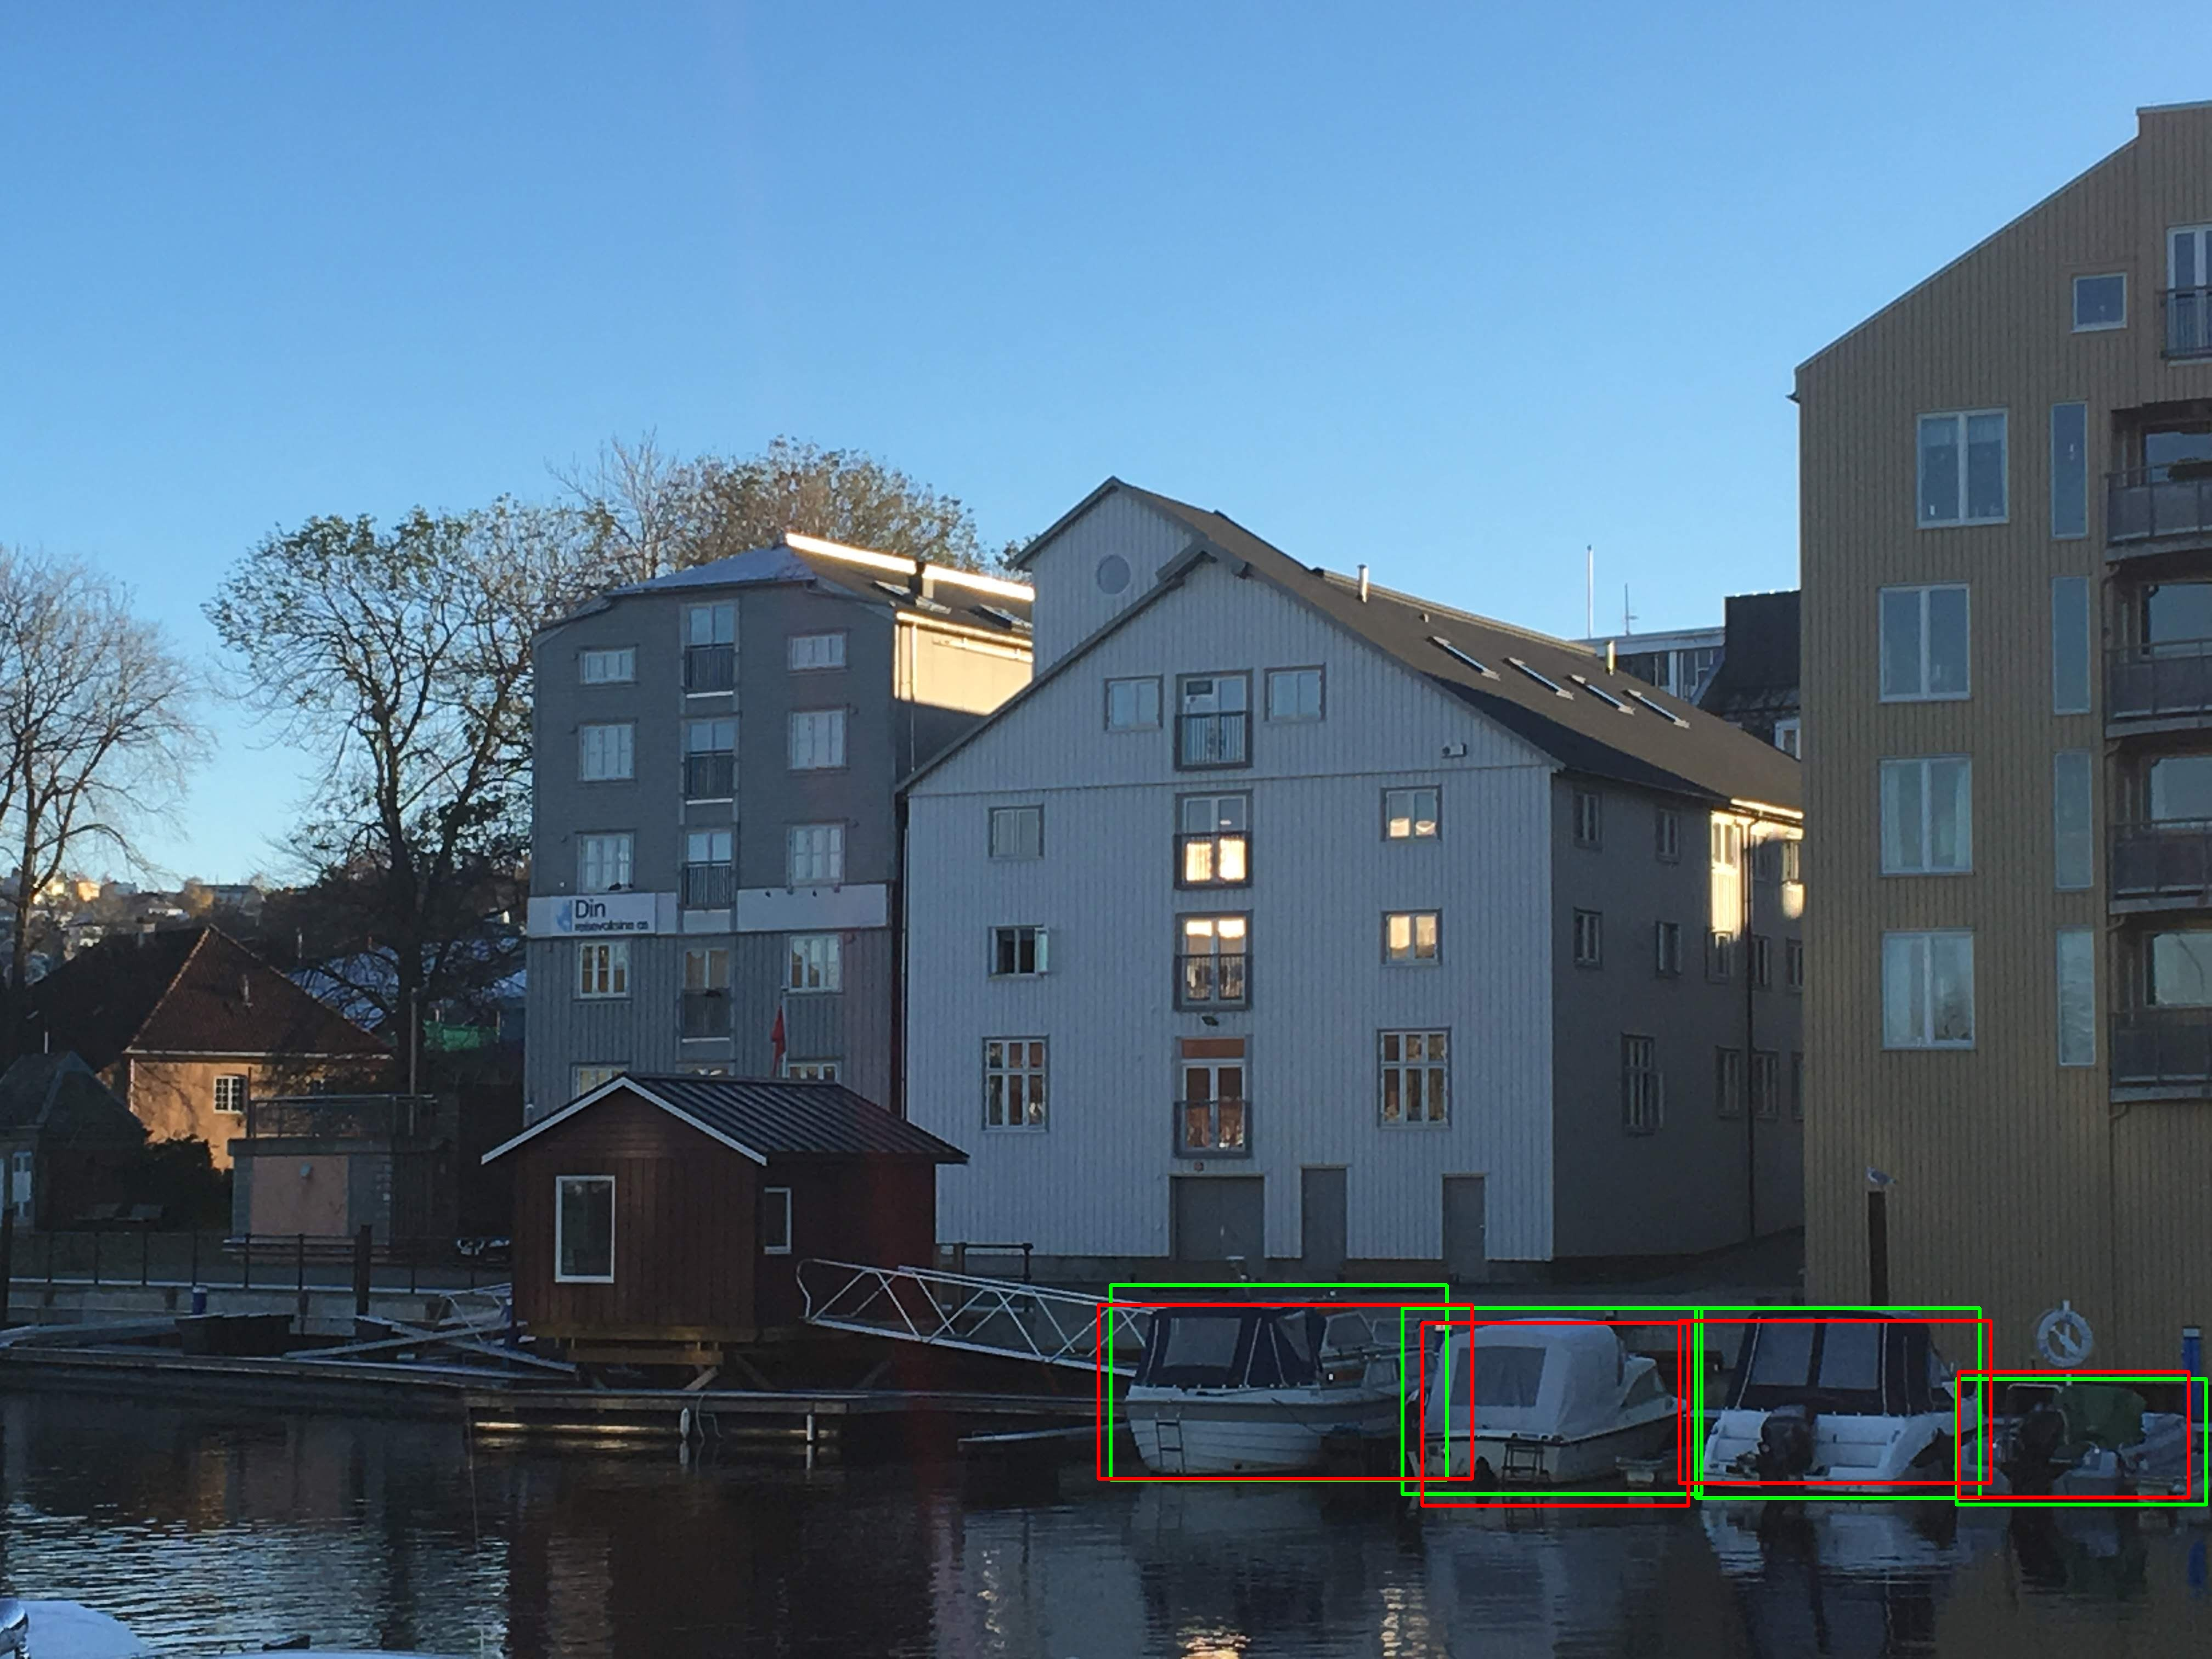
\includegraphics[width=0.8\linewidth]{results/case_buildings/prec_recall/yolo/IMG_2077_bbnb.jpg}
  \caption{Yolo2}
  \label{fig:ex_bbnb_yolo2}
\end{subfigure}%
\begin{subfigure}{.5\textwidth}
  \centering
  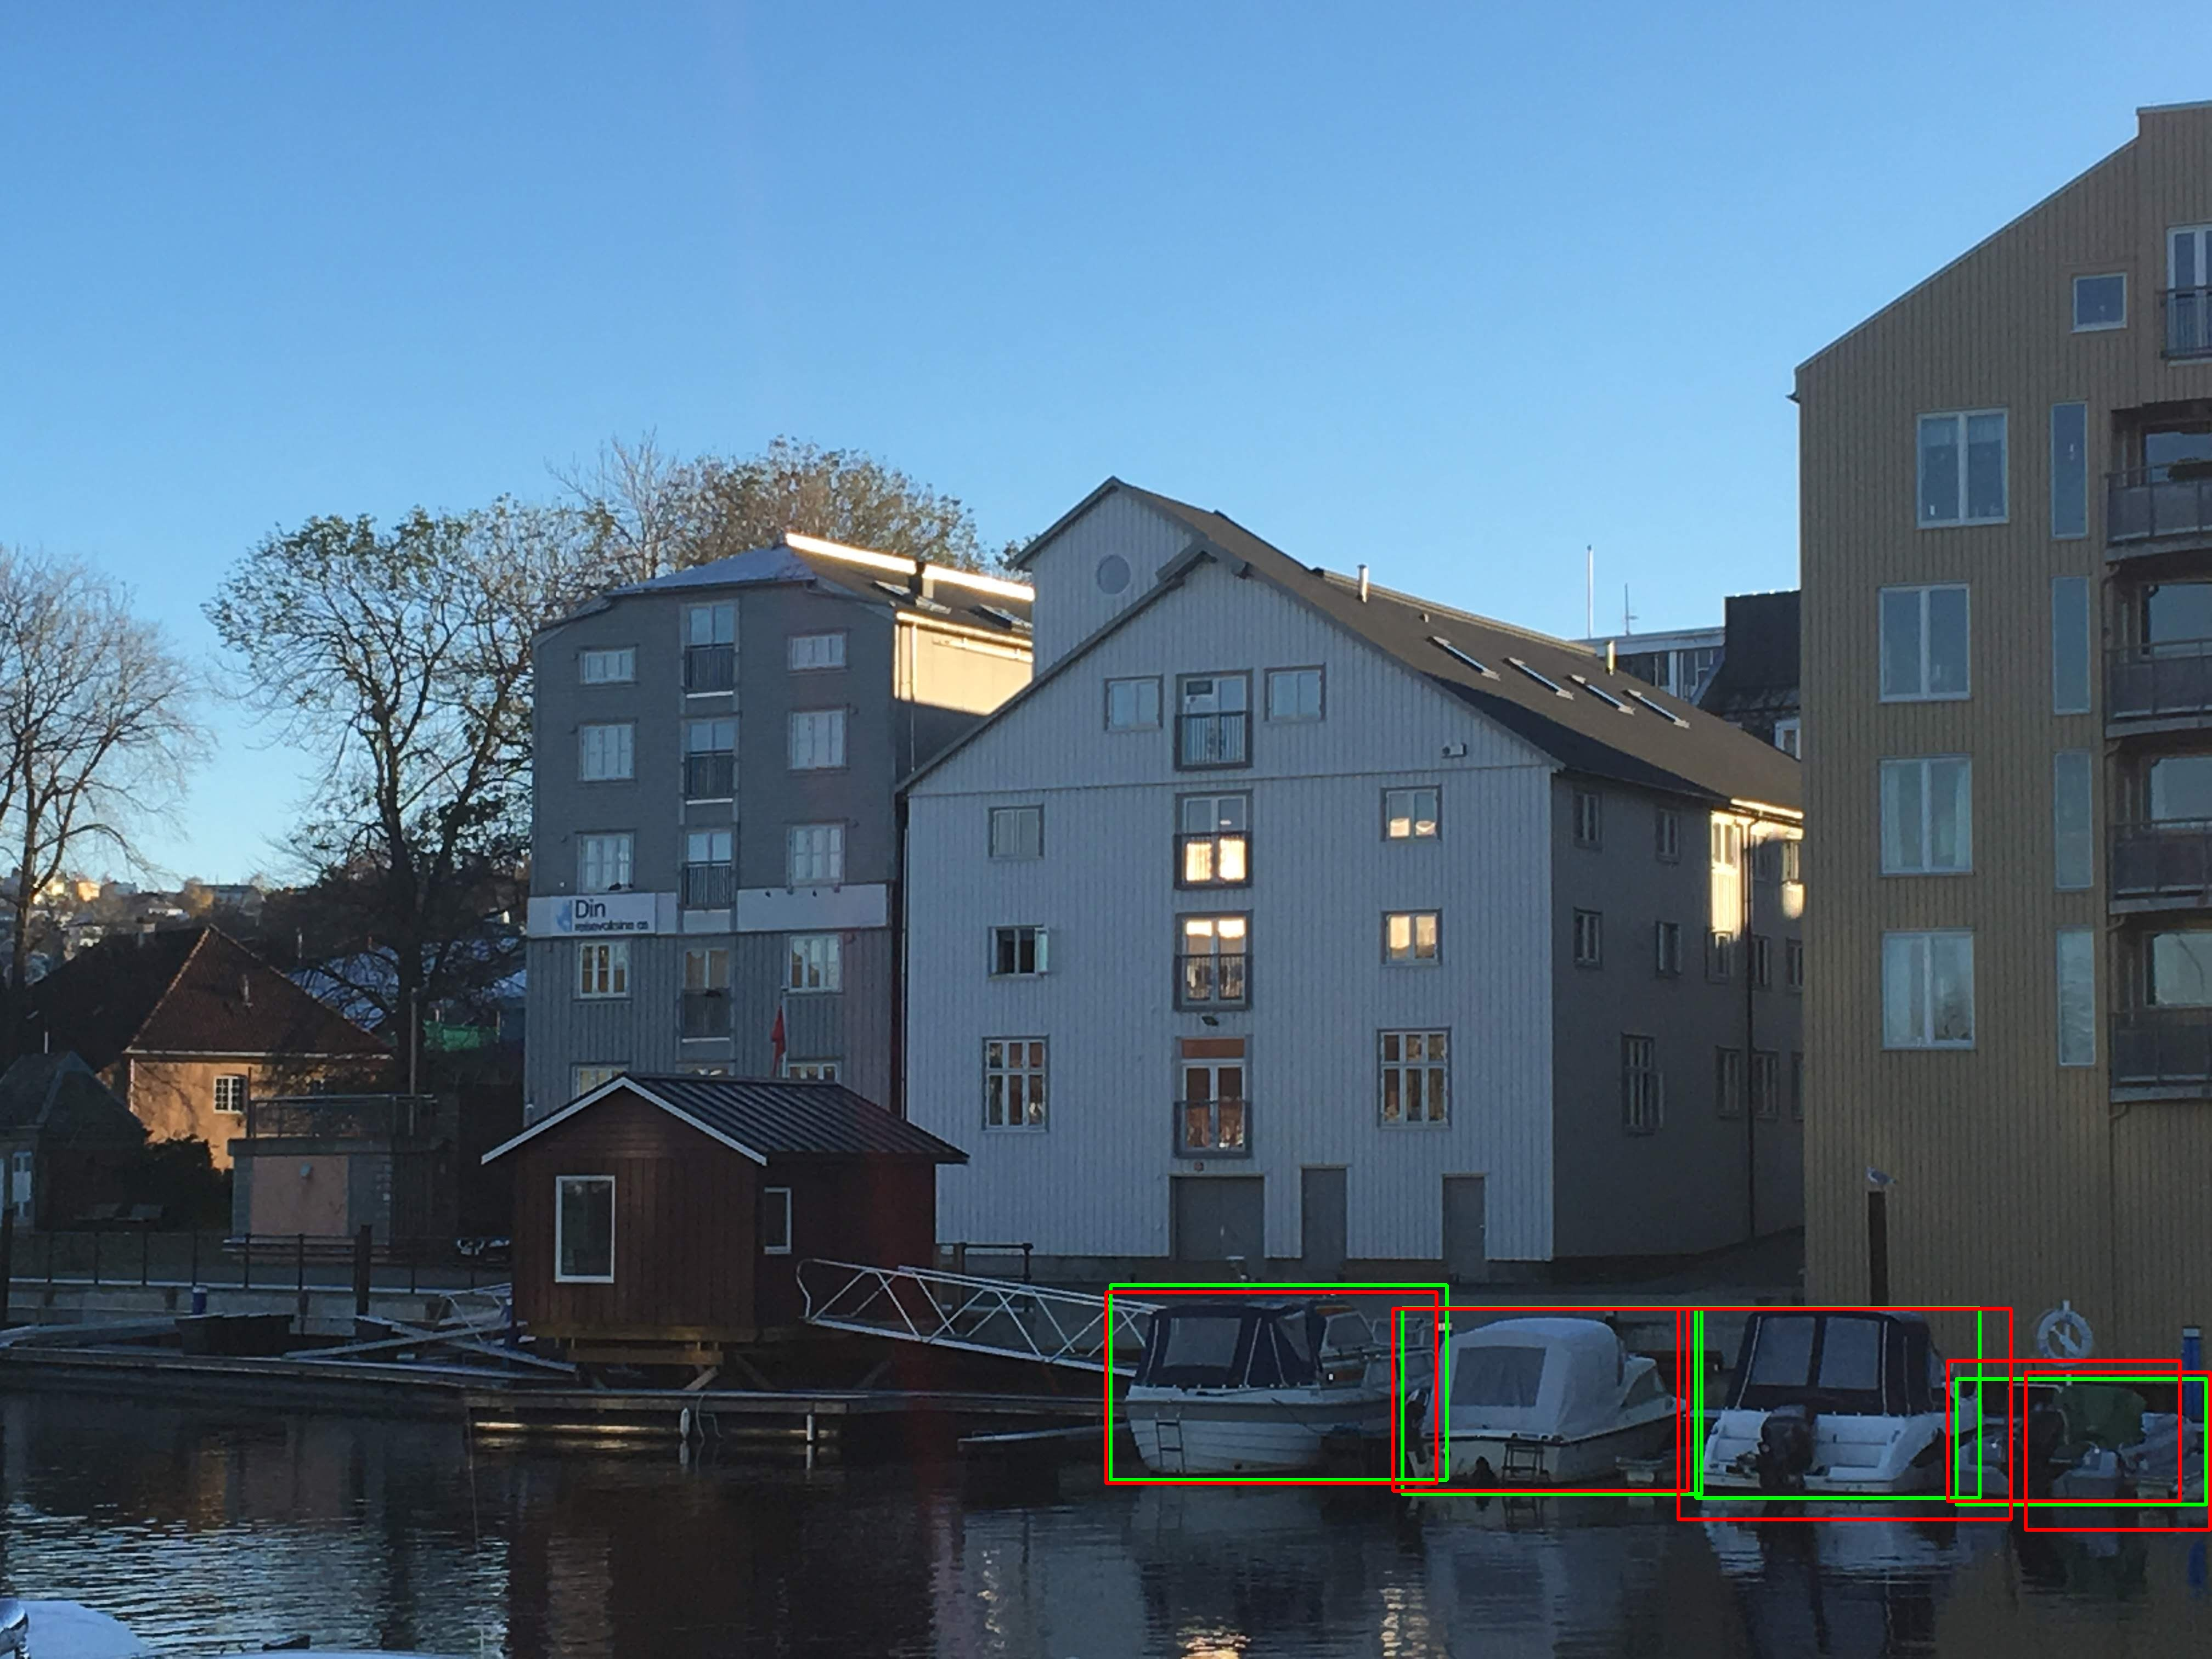
\includegraphics[width=.8\linewidth]{results/case_buildings/prec_recall/ssd/IMG_2077_bbnb.jpg}
  \caption{SSD2}
  \label{fig:ex_bbnb_ssd2}
\end{subfigure}

\begin{subfigure}{.5\textwidth}
  \centering
  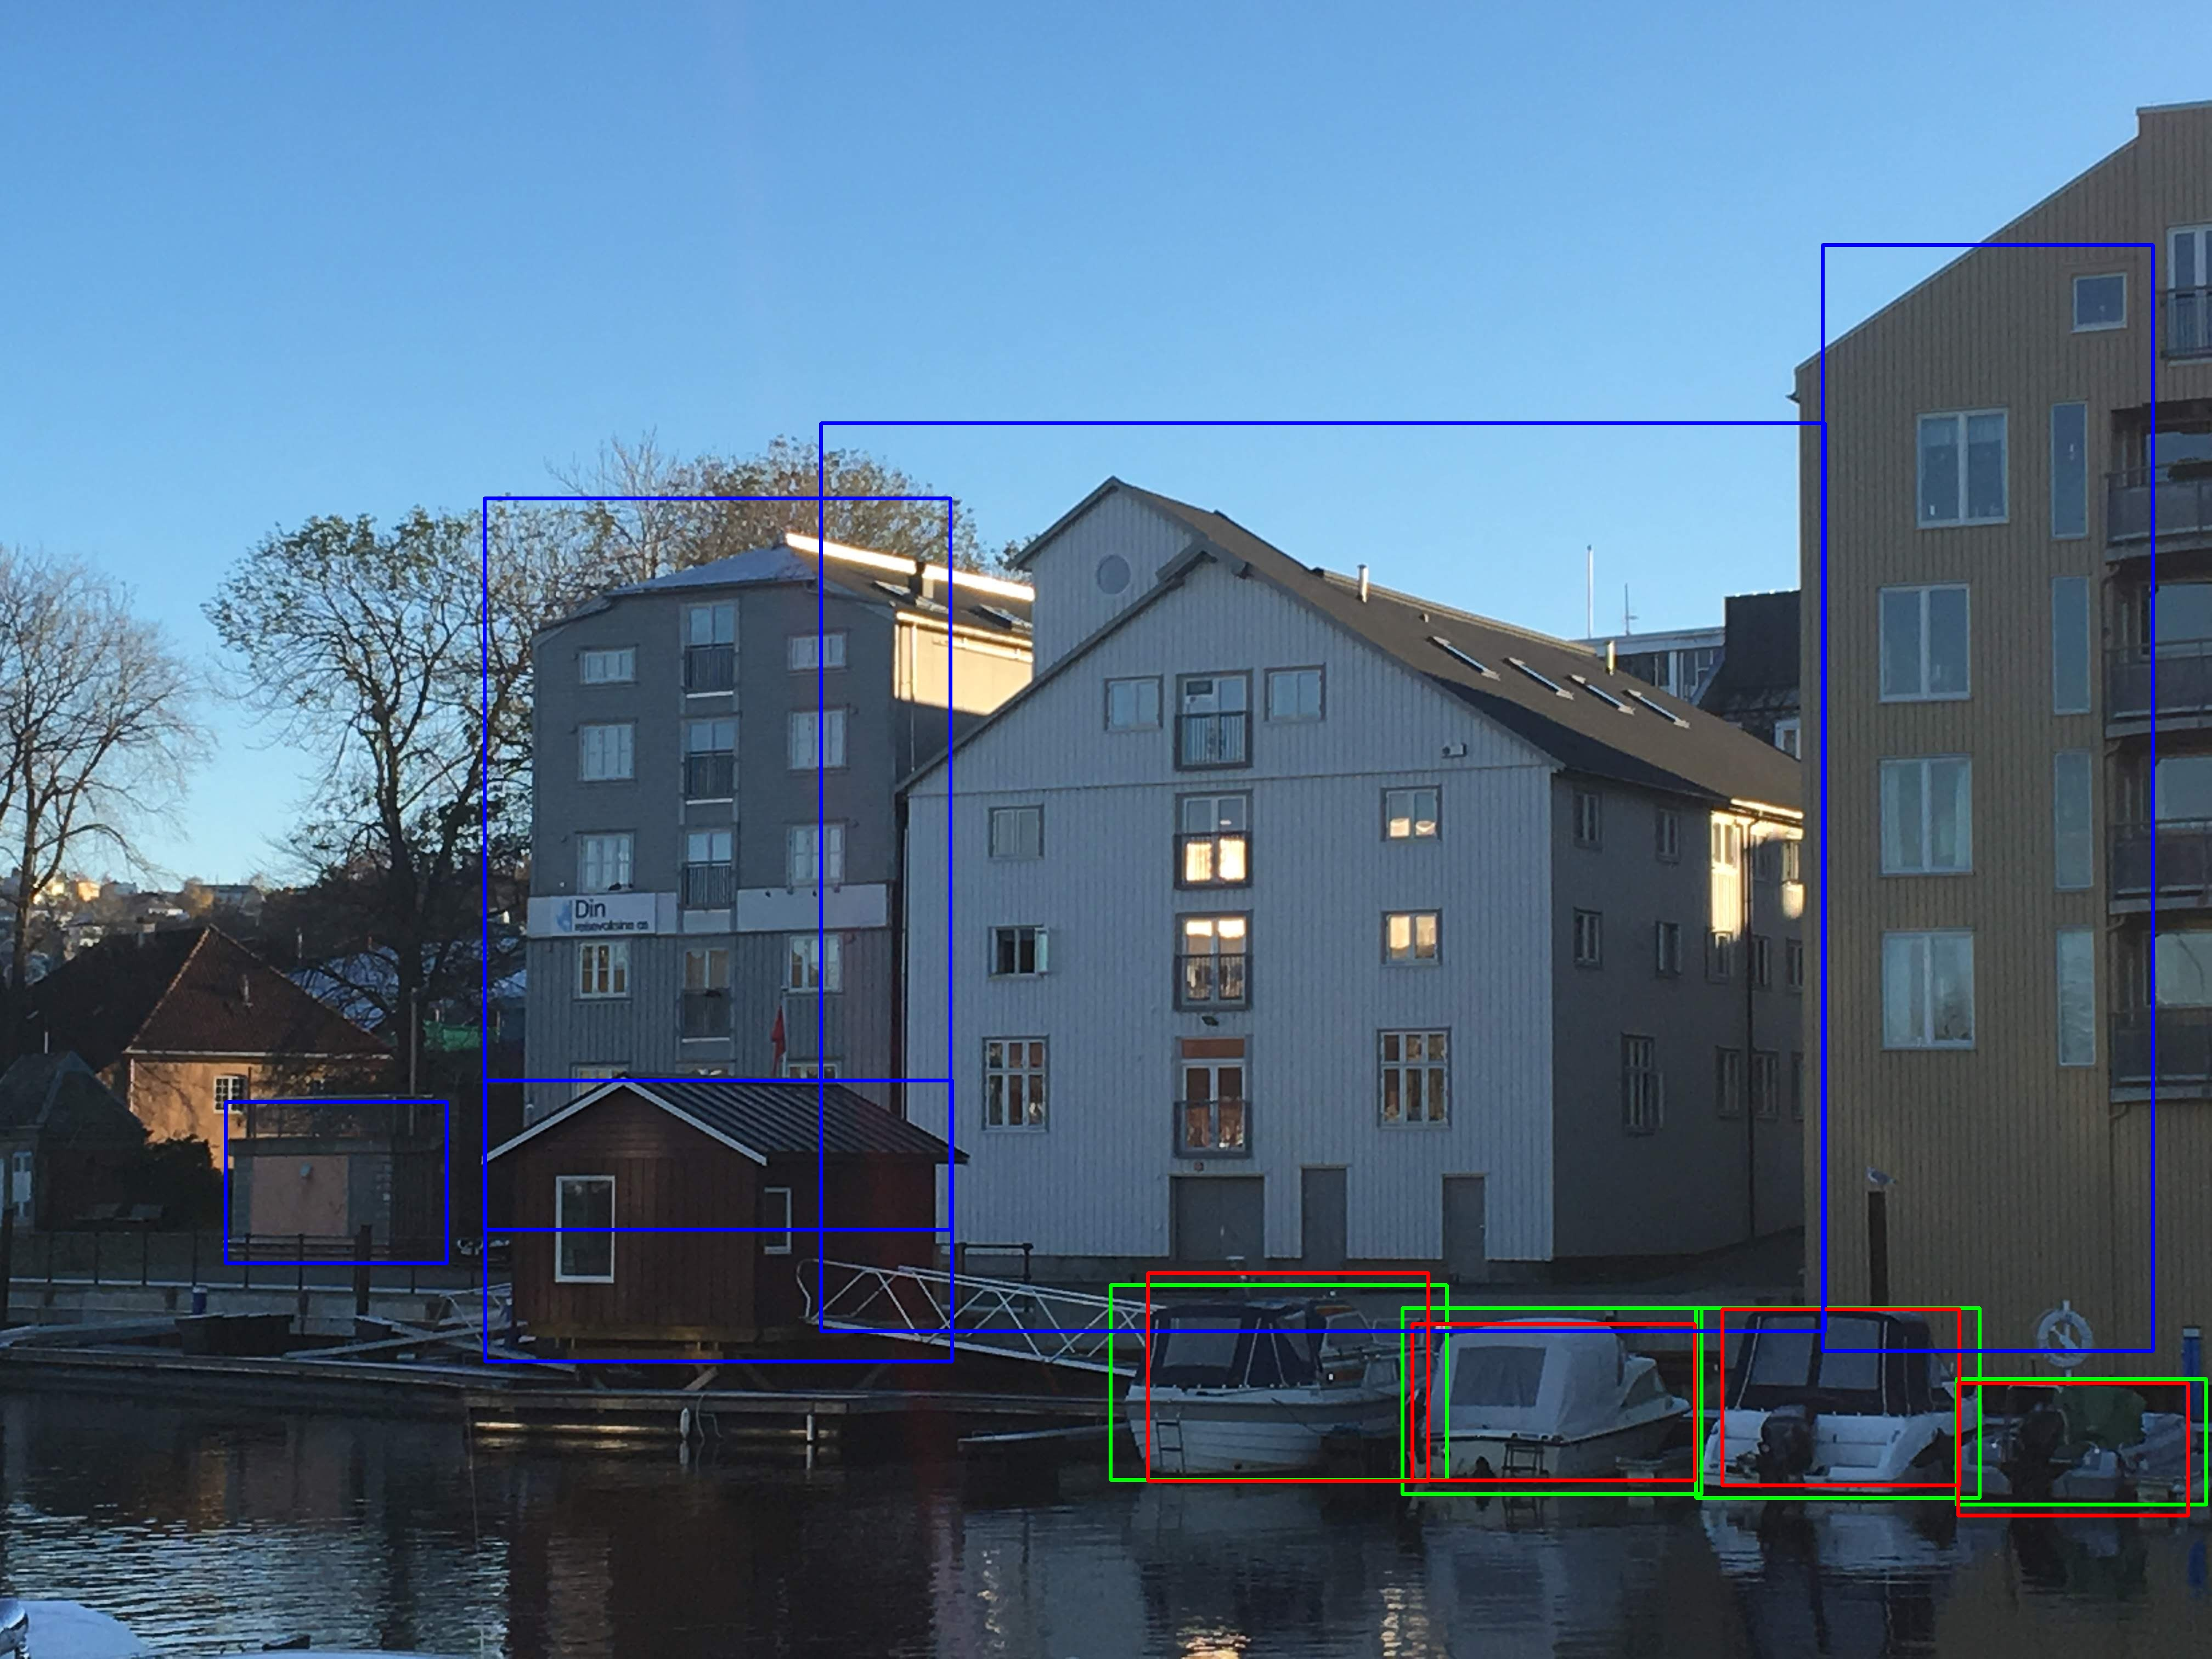
\includegraphics[width=0.8\linewidth]{results/case_buildings/prec_recall/yolo/IMG_2077_build.jpg}
  \caption{Yolo3}
  \label{fig:ex_bbnb_yolo3}
\end{subfigure}%
\begin{subfigure}{.5\textwidth}
  \centering
  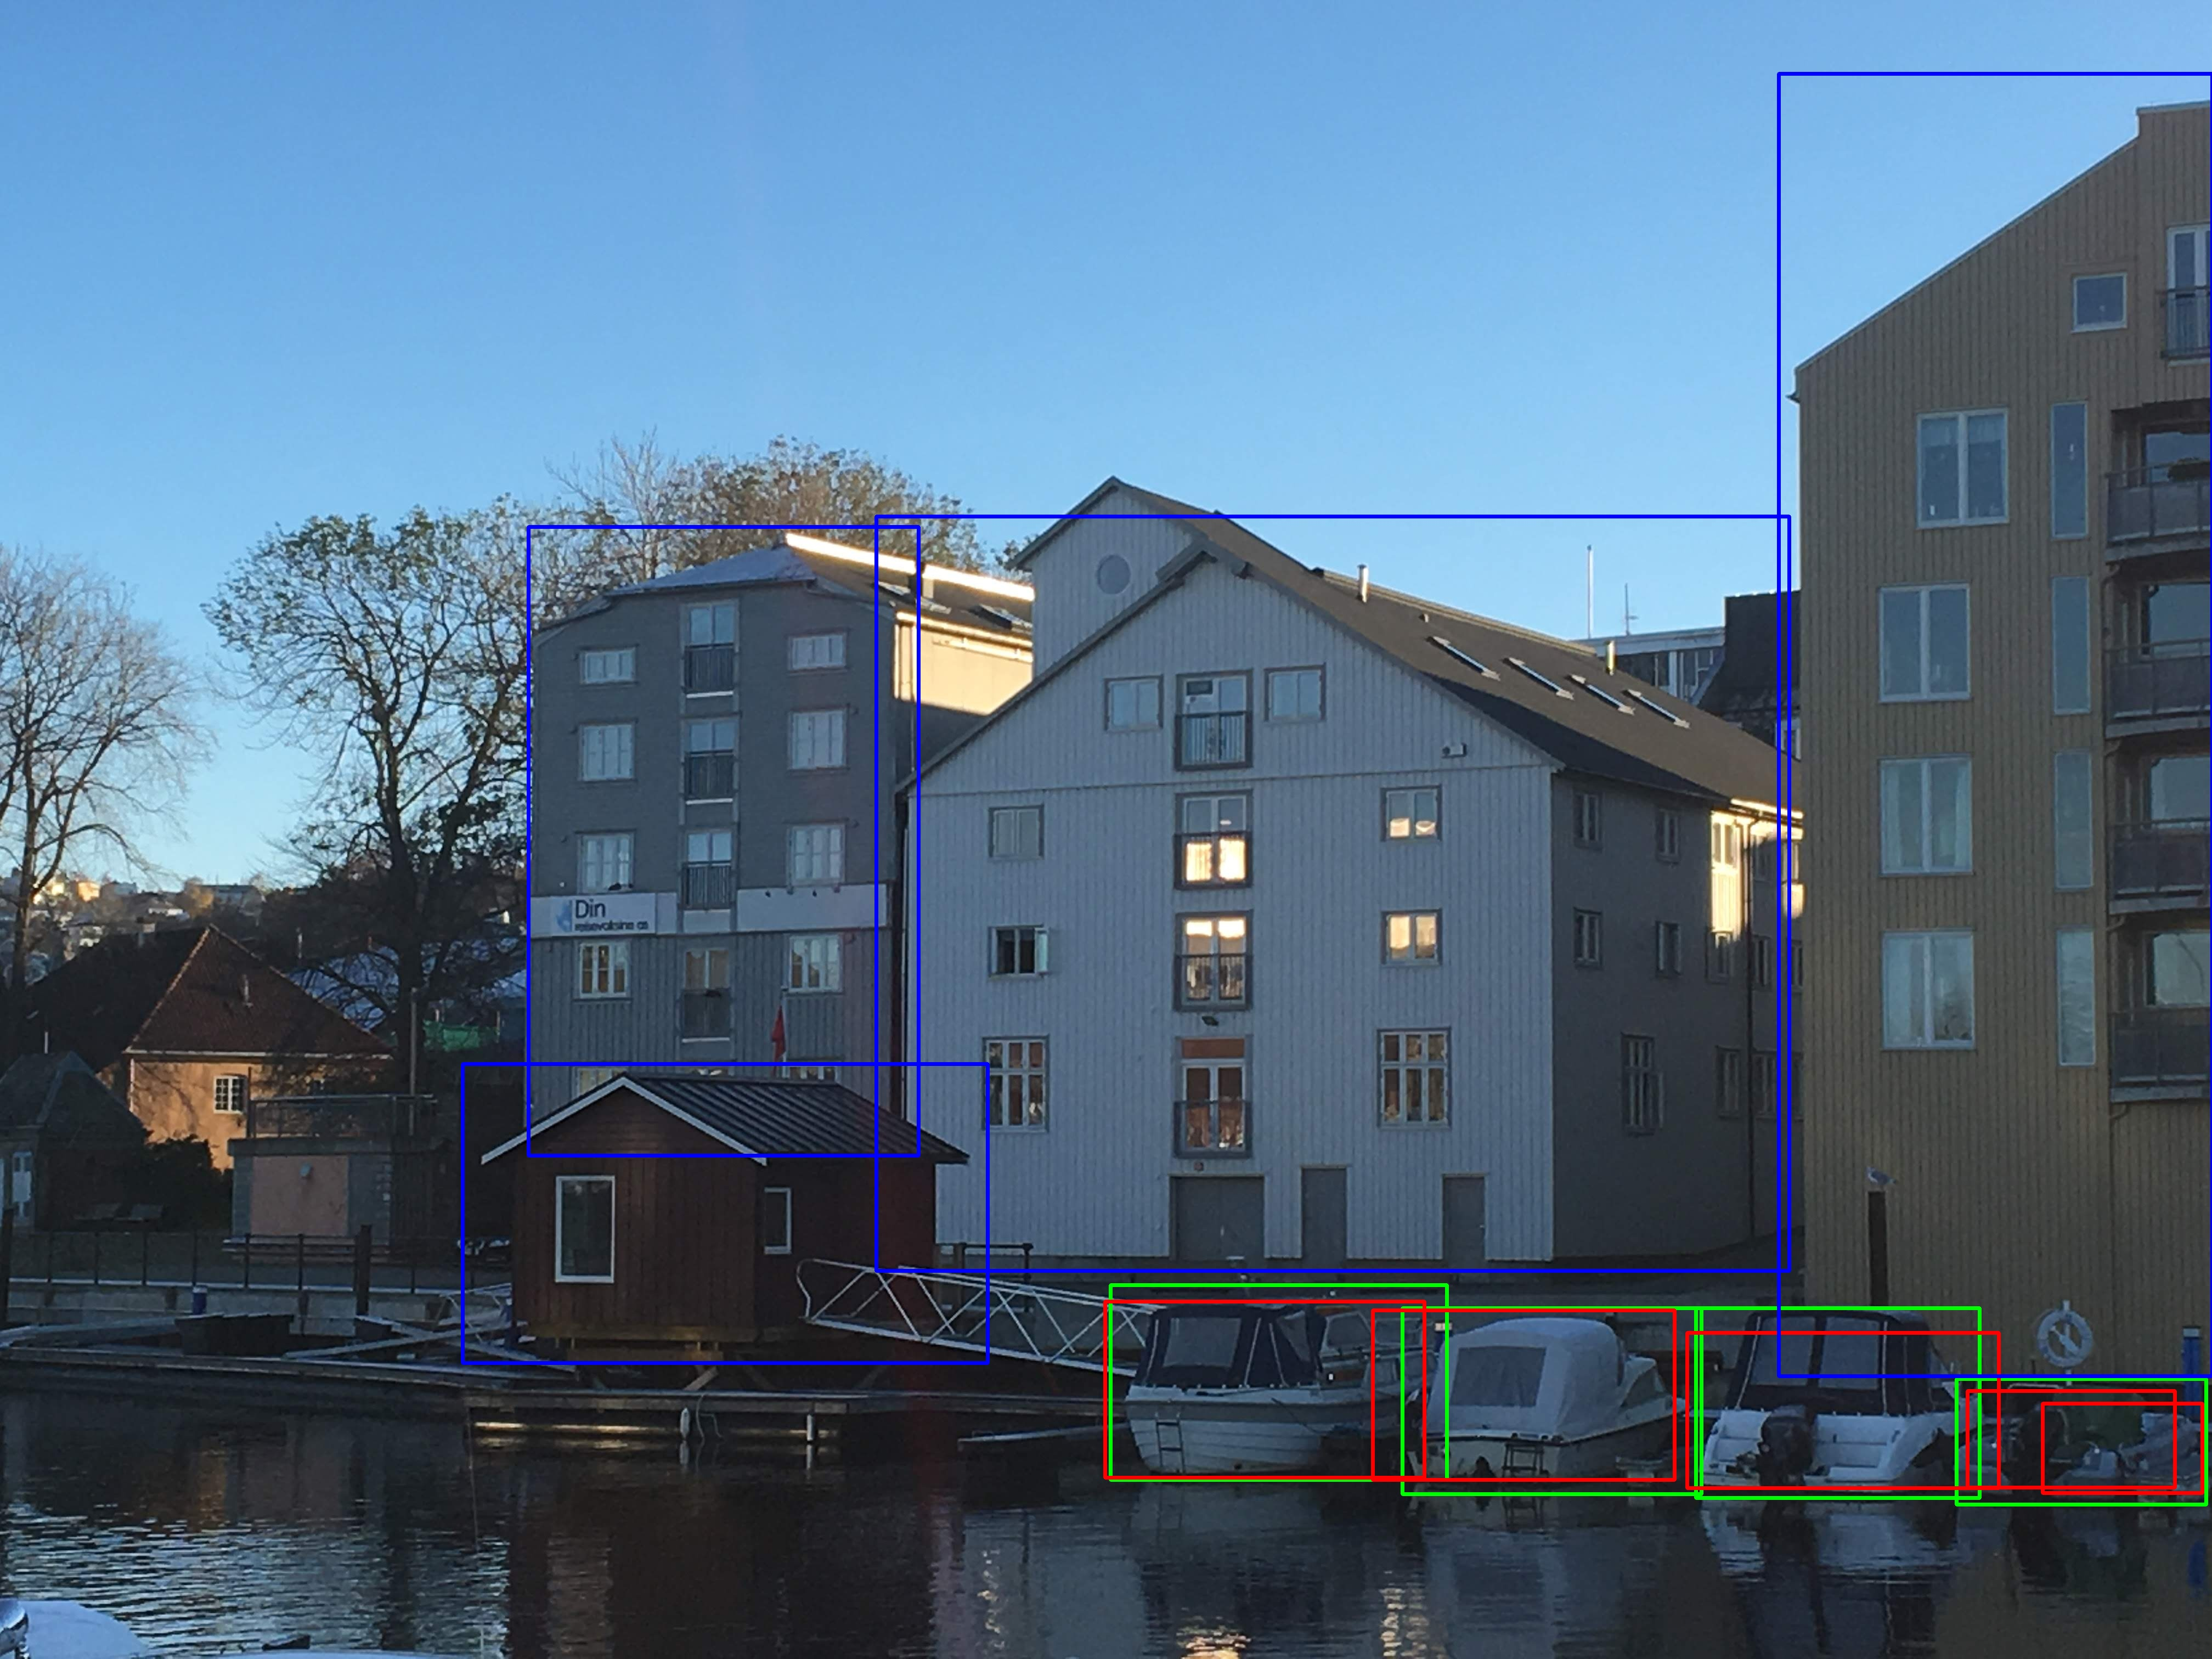
\includegraphics[width=.8\linewidth]{results/case_buildings/prec_recall/ssd/IMG_2077_build.jpg}
  \caption{SSD3}
  \label{fig:ex_bbnb_ssd3}
\end{subfigure}
\caption{Yolo2, Yolo3, SSD2, SSD3 example image from \textit{bbnb} test set. Green bounding boxes are ground truth, red bounding boxes are detected boats, blue bounding boxes are detected buildings}
\label{img:bbnb_ex}
\end{figure}





\newpage

\section{Video streaks}
\section{YOLO ssd}

